\documentclass[10pt,twoside,final]{book} % Use 10pt as specified, keep twoside from example

% --- Geometry Setup ---
\usepackage[paperwidth=7in, paperheight=10in,
            top=0.75in, bottom=0.75in,
            left=0.75in, right=0.75in, % Specification uses symmetric margins
            bindingoffset=0mm, % Explicitly set from spec
            headheight=45pt, % Keep from example for header space
            headsep=10pt,    % Keep from example
            twoside=true,    % Keep from example
            includehead=true,
            includefoot=true]{geometry}

% --- Packages ---
\usepackage[table]{xcolor}
\usepackage{tikz}
\usetikzlibrary{positioning,patterns}
\usepackage{tikzpagenodes} % Add this package
\usepackage{eso-pic}
\usepackage{fancyhdr}
\usepackage{titlesec}
\usepackage{mdframed}
\usepackage{graphicx}
\usepackage{fontspec} % Requires XeLaTeX or LuaLaTeX
\usepackage{fontawesome5}
\usepackage{setspace}
\usepackage{microtype}
\usepackage{ifthen}
\usepackage{amsmath}
\usepackage{amssymb}
\usepackage{calc} % Needed for width calculation
\usepackage{lipsum} % For placeholder text in examples if needed
\usepackage{framed} % For example boxes potentially
\usepackage{newverbs} % For verbatim examples

% --- FontAwesome Fix (From Example) ---
\usepackage{ifxetex,ifluatex}
\newif\ifxetexorluatex
\ifxetex
  \xetexorluatextrue
\else
  \ifluatex
    \xetexorluatextrue
  \else
    \xetexorluatexfalse
  \fi
\fi


\AddToShipoutPictureBG{%
  \begin{tikzpicture}[remember picture, overlay]
    % This line creates a clipping path. Anything drawn after this
    % will only be visible if it's inside the rectangle defined by the
    % bottom-left (south west) and top-right (north east) corners
    % of the main text area (the document body).
    \clip (current page text area.south west) rectangle (current page text area.north east);

    % --- Your original pattern drawing code ---
    % This code draws your large pattern as it did before.
    % However, because of the \clip command above, only the parts
    % of the pattern that fall within the document body will be shown.
    % The parts that would extend into the margins will be invisible.

    % Create a refined grid with proper offset for visual illusion
    \foreach \y in {-20,-19,...,60} {
      % Maintain the alternating offset crucial for the illusion
      \pgfmathsetmacro{\xoffset}{mod(\y,2)*0.4}
      \foreach \x in {-10,-9,...,30} {
        % Smaller dots but not too small to lose the effect
        \fill[gray!13] (\x*0.8cm + \xoffset cm, \y*0.8cm) circle (0.05cm);
      }
    }
    
    % Add subtle royal pattern at intersection points
    \foreach \yLoopVar in {-10,-8,...,30} {
      \foreach \xLoopVar in {-5,-3,...,15} {
        % Diamond pattern at key points - using pgfmath random function
        \pgfmathsetmacro{\randval}{random(1,100)}
        \ifdim\randval pt<10pt
          \fill[gray!15] (\xLoopVar*1.6cm, \yLoopVar*1.6cm+0.06cm) circle (0.03cm);
          \fill[gray!15] (\xLoopVar*1.6cm+0.06cm, \yLoopVar*1.6cm) circle (0.03cm);
          \fill[gray!15] (\xLoopVar*1.6cm, \yLoopVar*1.6cm-0.06cm) circle (0.03cm);
          \fill[gray!15] (\xLoopVar*1.6cm-0.06cm, \yLoopVar*1.6cm) circle (0.03cm);
        \fi
      }
    }
    % --- End of your original pattern drawing code ---
  \end{tikzpicture}%
}


% --- Font Setup (From Example - Requires User Path Update) ---
% !!! UPDATE FONT PATHS IF NECESSARY !!!
\setmainfont{CormorantGaramond}[
  Extension=.otf,
  UprightFont=*-Regular,
  BoldFont=*-Bold,
  ItalicFont=*-Italic,
  BoldItalicFont=*-BoldItalic,
  Path = /home/nick/.local/share/fonts/ % <<<--- EXAMPLE PATH - UPDATE THIS!!!
]
\setsansfont{Montserrat}[
  Extension=.otf,
  UprightFont=*-Regular,
  BoldFont=*-Bold,
  Path = /home/nick/.local/share/fonts/ % <<<--- EXAMPLE PATH - UPDATE THIS!!!
]

% --- Spacing (From Example) ---
\setlength{\parskip}{0.5em}
\setlength{\parindent}{0pt}
\onehalfspacing

% --- Color Definitions (B&W Grayscale Optimized) ---
\definecolor{graydarker}{gray}{0.15} % Very Dark Gray (almost black)
\definecolor{graydark}{gray}{0.35}  % Dark Gray
\definecolor{graymedium}{gray}{0.65} % Medium Gray
\definecolor{graylight}{gray}{0.85}  % Light Gray
\definecolor{grayverylight}{gray}{0.96} % Very Light Gray (near white)
\definecolor{linecolor}{gray}{0.75}   % Gray for lines

% --- Reassign Theme Colors ---
\colorlet{rvprimary}{graydark}      % Use Dark Gray for primary elements
\colorlet{rvsecondary}{graymedium} % Use Medium Gray for secondary elements
\colorlet{rvaccent}{graydarker}    % Use Very Dark Gray for accents (like rules/titles)
\colorlet{rvlight}{grayverylight} % Use Very Light Gray for backgrounds
\colorlet{headercolor}{grayverylight} % Background for headers
\colorlet{titlecolor}{graydarker}    % Title text color
\colorlet{quotecolor}{graylight}    % Background for quote boxes

% --- Adjust Text Colors for Contrast ---
\colorlet{frametitletextcolor}{white}       % Text color for dark frame titles (rvprimary/rvaccent)
\colorlet{frametitlesecondarytextcolor}{black} % Text color for lighter frame titles (rvsecondary - now graymedium)


% --- Icons (From Specification + Example) ---
\newcommand{\rvicon}[1]{\textcolor{rvprimary}{\large\faIcon{#1}}}
\newcommand{\targeticon}{\rvicon{bullseye}}
\newcommand{\protocolicon}{\rvicon{clipboard-list}}
\newcommand{\analysisicon}{\rvicon{chart-line}}
\newcommand{\insighticon}{\rvicon{lightbulb}}
\newcommand{\progressicon}{\rvicon{chart-bar}}
\newcommand{\pencilicon}{\rvicon{pen}} % Borrowed
\newcommand{\clockicon}{\rvicon{clock}} % Borrowed
\newcommand{\eyeicon}{\rvicon{eye}} % Borrowed
\newcommand{\checkicon}{\rvicon{clipboard-check}} % Borrowed, remapped
\newcommand{\reviewicon}{\rvicon{tasks}} % Borrowed/Renamed
\newcommand{\milestoneicon}{\rvicon{trophy}} % Borrowed/Renamed
\newcommand{\mapicon}{\rvicon{map-marked-alt}} % Borrowed/Renamed
\newcommand{\bookicon}{\rvicon{book-open}} % Borrowed/Renamed
\newcommand{\infoicon}{\rvicon{info-circle}} % Added
\newcommand{\exampleicon}{\rvicon{vial}} % Added
\newcommand{\cautionicon}{\rvicon{exclamation-triangle}} % Added
\newcommand{\concepticon}{\rvicon{project-diagram}} % Added

  \newlength{\labelwidthA}
  \newlength{\labelwidthB}
  \newlength{\labelwidthC}
% --- Custom Symbol (From Example - Requires User Path Update) ---
% !!! UPDATE SYMBOL PATH IF NECESSARY !!!
\newcommand{\themesymbol}{%
  \includegraphics[height=15pt]{shadow-symbol.png}% % <<<--- UPDATE PATH IF NEEDED
}

% --- Headers (Adapted from Example) ---
\pagestyle{fancy}
\fancyhf{}
\fancyhead[LE,RO]{\themesymbol~\thepage}
\fancyhead[RE,LO]{\textit{\small\journaltitle}} % Needs \journaltitle defined
\renewcommand{\headrulewidth}{0.5pt}
\renewcommand{\headrule}{\hbox to\headwidth{%
  \color{rvprimary}\leaders\hrule height \headrulewidth\hfill}}

% --- Journal Configuration ---
\newcommand{\journaltitle}{REMOTE VIEWING}
\newcommand{\journalsubtitle}{A 90-Day Guided Protocol Based on Declassified CIA Stargate Methods}
\newcommand{\journalfootertext}{Train Your Mind, Expand Your Perception} % Added for consistency

% --- Title Formatting (Corrected Simplified Version) ---
\titleformat{\chapter}[display]
  {\normalfont\huge\bfseries\centering\color{titlecolor}} % Formatting for the title text itself
  {} % Clear the label format
  {0pt} % Separation between label and title
  {% Code executed before the title is typeset
    \ifnum\value{chapter}>0 % Check if it's a numbered chapter (not \chapter*)
      \centering % Center the label
      {\Large \vspace*{-20pt} % Move label up slightly
       \MakeUppercase{\chaptername}~\thechapter} % Use \chaptername (might be CHAPTER or APPENDIX)
      \vspace{25pt} % Space after the label before the title
      \centering % Re-assert centering for the title itself if needed
    \fi
  }
\titlespacing*{\chapter}{0pt}{10pt}{40pt} % Reduced top spacing slightly due to manual label space

% --- Customize Appendix Chapter Name ---
\usepackage{apptools}
\AtAppendix{\renewcommand{\chaptername}{APPENDIX}} % Change "Chapter" to "APPENDIX" for appendix chapters


% --- Decorative Element (Adapted from Example) ---
\newcommand{\themedecoration}{%
  \begin{center}
    \themesymbol
  \end{center}%
}

% --- Section Divider (Adapted from Example) ---
\newcommand{\elegantdivider}{%
  \begin{center}
    \textcolor{rvprimary}{\rule{0.3\textwidth}{0.7pt}}%
    \themesymbol%
    \textcolor{rvprimary}{\rule{0.3\textwidth}{0.7pt}}%
  \end{center}
}

% --- Custom Environments (From Specification, Styled like Example) ---
% Base style for RV boxes
\mdfdefinestyle{rvBaseStyle}{%
  linewidth=0.7pt,
  roundcorner=5pt,
  innertopmargin=10pt,
  innerbottommargin=10pt,
  innerleftmargin=10pt,
  innerrightmargin=10pt,
  shadow=true,
  shadowsize=1pt,
}

% RV Session Box (Updated Title)
\newmdenv[
  style=rvBaseStyle,
  linecolor=rvprimary, backgroundcolor=white,
  frametitle={Impressions \& Perceptions}, % Ampersand escaped
  frametitlebackgroundcolor=rvprimary,
  frametitlefont=\color{frametitletextcolor}\bfseries\Large,
  frametitlealignment=\centering,
  shadowcolor=graydark!40, % Explicit gray shade
]{rvSessionBox}

% RV Protocol Box
\newmdenv[
  style=rvBaseStyle,
  linecolor=rvaccent, backgroundcolor=rvlight,
  frametitle={Today's Protocol},
  frametitlebackgroundcolor=rvaccent,
  frametitlefont=\color{frametitletextcolor}\bfseries\Large,
  frametitlealignment=\centering,
  shadowcolor=graydarker!40, % Explicit gray shade
]{rvProtocolBox}

% RV Target Practice Box (Updated Text Color)
\newmdenv[
  style=rvBaseStyle,
  linecolor=rvsecondary, backgroundcolor=white,
  frametitle={Target Practice},
  frametitlebackgroundcolor=rvsecondary,
  frametitlefont=\color{frametitlesecondarytextcolor}\bfseries\Large, % Black text on medium gray
  frametitlealignment=\centering,
  shadowcolor=graymedium!60, % Explicit gray shade
]{rvTargetBox}

% RV Analysis Box (Updated Title)
\newmdenv[
  style=rvBaseStyle,
  linecolor=rvprimary, backgroundcolor=white,
  frametitle={Session Analysis (Complete Post-Verification)},
  frametitlebackgroundcolor=rvprimary,
  frametitlefont=\color{frametitletextcolor}\bfseries\Large,
  frametitlealignment=\centering,
  shadowcolor=graydark!40, % Explicit gray shade
]{rvAnalysisBox}

% Quote Box (Adapted from Example)
\newenvironment{quotebox}
  {\begin{mdframed}[
    topline=true, bottomline=true, leftline=false, rightline=false,
    linewidth=0.5pt, linecolor=rvaccent, % Use accent color (darker gray)
    backgroundcolor=quotecolor, % Use light gray background
    shadow=true, shadowsize=1pt, shadowcolor=graydarker!30, % Use darker shadow
    innertopmargin=10pt, innerbottommargin=10pt
  ]
    \centering\small\itshape}
  {\end{mdframed}}

% Journal Prompt Box (Adapted from Example - simple intro/guidance)
\newenvironment{journalprompt}
  {\begin{mdframed}[
    backgroundcolor=rvlight, linewidth=0.7pt, linecolor=rvprimary,
    shadow=true, shadowsize=1pt, shadowcolor=graydark!40,
    roundcorner=3pt, innertopmargin=10pt, innerbottommargin=10pt,
    leftmargin=5pt, rightmargin=5pt
  ]
  \itshape}
  {\end{mdframed}}

% General Framed Box for Reviews/Milestones (From Spec)
\newenvironment{reviewbox}[1]
 {\begin{mdframed}[
    linecolor=rvprimary, backgroundcolor=white, roundcorner=5pt,
    linewidth=0.7pt, shadow=true, shadowsize=1pt, shadowcolor=graydark!40,
    frametitle={#1}, frametitlebackgroundcolor=rvprimary,
    frametitlefont=\color{frametitletextcolor}\bfseries\Large,
    frametitlealignment=\centering
  ]}
  {\end{mdframed}}

\newenvironment{milestonebox}[1]
 {\begin{mdframed}[
    linecolor=rvaccent, backgroundcolor=white, roundcorner=5pt,
    linewidth=0.7pt, shadow=true, shadowsize=2pt, shadowcolor=graydarker!40,
    frametitle={#1}, frametitlebackgroundcolor=rvaccent,
    frametitlefont=\color{frametitletextcolor}\bfseries\Large,
    frametitlealignment=\centering
  ]}
  {\end{mdframed}}

% Box style for concept introductions
\mdfdefinestyle{conceptStyle}{%
  linecolor=rvprimary, backgroundcolor=white, roundcorner=5pt,
  linewidth=0.7pt, shadow=true, shadowsize=1pt, shadowcolor=graydark!40,
  innertopmargin=\topskip, innerbottommargin=\topskip,
  innerleftmargin=10pt, innerrightmargin=10pt,
  frametitlebackgroundcolor=rvprimary,
  frametitlefont=\color{frametitletextcolor}\bfseries\Large,
  frametitlealignment=\centering
}

% Box style for examples within concept introductions
\mdfdefinestyle{exampleStyle}{%
  linecolor=rvsecondary, backgroundcolor=rvlight, roundcorner=3pt,
  linewidth=0.5pt, shadow=false,
  innertopmargin=5pt, innerbottommargin=5pt,
  innerleftmargin=8pt, innerrightmargin=8pt,
  frametitlebackgroundcolor=rvsecondary,
  frametitlefont=\color{frametitlesecondarytextcolor}\bfseries\normalsize, % Smaller title
  frametitlealignment=\centering
}

% --- Commands for Lined Sections ---
\newcommand{\linedspace}[1]{% Number of lines
    \vspace{0.2cm} % Space before lines
    \foreach \n in {1,...,#1}{%
        \noindent\textcolor{linecolor!70}{\rule{\textwidth}{0.3pt}}\\[0.9\baselineskip]% Adjust line spacing if needed
    }
    \vspace{0.1cm} % Space after lines
}

% --- Page Templates ---

% Daily Entry Page (With Analysis Box Fix)
\newcommand{\journaldayrv}[4]{ % #1=Day, #2=Protocol Text, #3=Target Text, #4=Quote
\clearpage
\begin{center}
\Large\textbf{\color{titlecolor}DAY #1}\\[0.3cm]
\tikz\node[draw=rvprimary, line width=0.6pt, inner sep=5pt, rounded corners=2pt]{\normalfont\small\textcolor{titlecolor}{Date: \rule{2in}{0.4pt}}}; % Date line
\end{center}
\vspace{0.4cm}

\begin{rvProtocolBox}
  \protocolicon~\textbf{Focus:} #2 % Protocol instructions here
\end{rvProtocolBox}
\vspace{0.4cm}

\begin{rvTargetBox}
  \targeticon~\textbf{Target Details:} #3 % Target info here
\end{rvTargetBox}
\vspace{0.4cm}

\begin{rvSessionBox} % Title now has escaped ampersand
  \linedspace{15} % Adjust number of lines as needed for impressions/sketches
\end{rvSessionBox}
\vspace{0.4cm}

% --- Corrected Analysis Box Content (Restoring Lines using \textwidth) ---
\begin{rvAnalysisBox}
  \analysisicon~\textbf{Assessment:}\\[0.3cm] % Icon present
  Accuracy: $\square$ Low \quad $\square$ Medium \quad $\square$ High \quad $\square$ N/A (Practice)\\[0.5cm]

  \checkicon~\textbf{Key Successful Elements / Correct Perceptions:} 
  
    \vspace{0.1cm}     
    \foreach \n in {1,...,4}{
        \noindent\textcolor{linecolor!70}{\rule{\textwidth}{0.3pt}}\\[0.9\baselineskip]
    }
    \vspace{0.1cm} % Space after lines

  \cautionicon~\textbf{Areas for Improvement / Analytical Overlay (AOL):} 
  
    \vspace{0.2cm} % Space before lines
    \foreach \n in {1,...,4}{% Adjust number of lines if needed
        \noindent\textcolor{linecolor!70}{\rule{\textwidth}{0.3pt}}\\[0.9\baselineskip]
    }
    \vspace{0.1cm} % Space after lines

  \insighticon~\textbf{Insights Gained / Surprising Elements:} 
  
    \vspace{0.2cm} % Space before lines
    \foreach \n in {1,...,4}{% Adjust number of lines if needed
        \noindent\textcolor{linecolor!70}{\rule{\textwidth}{0.3pt}}\\[0.9\baselineskip]
    }
    \vspace{0.1cm} % Space after lines
\end{rvAnalysisBox}
% --- End of Corrected Analysis Box Content ---
\vspace{0.4cm}

\begin{quotebox}
#4 % Quote
\end{quotebox}
}

% Weekly Review Page (No changes needed from previous fix)
\newcommand{\weeklyreviewrv}[1]{ % #1=Week Number
\clearpage
\begin{center}
\Large\textbf{\color{titlecolor}WEEK #1 REVIEW \reviewicon}\\[0.3cm]
\elegantdivider
\end{center}
\vspace{0.4cm}
\begin{journalprompt}
Reflect on your remote viewing practice this past week. Review your session notes, paying attention to accuracy, common types of perceptions (visual, sensory, emotional, symbolic), and any interference from your analytical mind (AOL).
\end{journalprompt}
\vspace{0.4cm}
\begin{reviewbox}{Weekly Progress Summary}
  \progressicon~\textbf{Overall Progress:} Note general feelings about development, consistency of practice, mindset.\linedspace{4}
  \targeticon~\textbf{Most Successful Session(s) \& Key Hits:} Describe sessions that felt accurate or yielded verifiable data.
  
  \linedspace{4}
  \eyeicon~\textbf{Patterns Noticed:} Identify recurring types of perceptions, common errors, or types of AOL.
  
  \linedspace{4}
  \pencilicon~\textbf{Techniques/Areas to Focus On Next Week:} What specific protocol stages or mindset aspects need refinement?
  
  \linedspace{4}
\end{reviewbox}
\vspace{0.3cm}
\begin{quotebox}
"The only source of knowledge is experience." — Albert Einstein % Example Quote
\end{quotebox}
}

% Milestone Page (No changes needed from previous fix)
\newcommand{\milestonerv}[3]{ % #1=Day Number, #2=Milestone Title Text, #3=Quote Text
\clearpage
\begin{center}
\vspace*{0.5cm}
{\Huge\bfseries\color{titlecolor} MILESTONE: DAY #1 \milestoneicon}\\[0.4cm]
\includegraphics[width=2in]{shadow-symbol.png}\\[0.4cm] % <<<--- UPDATE PATH IF NEEDED
{\Large\itshape Honoring Your Remote Viewing Progress}
\end{center}
\vspace{0.5cm}
\begin{milestonebox}{#2} % Milestone subtitle passed as argument
\begin{center}
Acknowledge your dedication to learning this structured approach to perception. This journey requires discipline, patience, and openness. Reflect on your development over the past 30 days.
\end{center}

\vspace{0.3cm}
\progressicon~\textbf{Three most significant improvements in my remote viewing abilities:}

\linedspace{4}


\insighticon~\textbf{Most surprising perceptions or accurate hits during this phase:}

\linedspace{4} 

\mapicon~\textbf{My intentions for the next phase of training:}

\linedspace{4}  

\end{milestonebox}
\vspace{0.4cm}
\begin{quotebox}
#3 % <<< Use the third argument for the quote
\end{quotebox}
\vspace{0.5cm}
\themedecoration
}

% Skill Tracker Page (No changes needed from previous fix)
\newcommand{\skilltracker}{
\clearpage
\chapter*{REMOTE VIEWING SKILL TRACKER}
\thispagestyle{fancy} % Ensure header appears
\begin{center}
\Large\itshape Track Your Developing Abilities
\vspace{0.2cm}
\elegantdivider
\end{center}
\vspace{0.4cm}
\begin{reviewbox}{Skill Development Grid}
Use this grid to mark your perceived proficiency as you progress. Check the box corresponding to the phase where you feel you started developing or achieved proficiency in each skill area. This is subjective; update it as you review your progress.
\vspace{0.5cm}
\centering
\resizebox{\textwidth}{!}{% Resize table to fit width
\begin{tabular}{|p{3cm}|p{2.7cm}|p{3cm}|p{2.7cm}|p{2.7cm}|} % Adjusted widths slightly
\hline
\rowcolor{rvprimary!15} % Light header row (adjust gray intensity if needed)
\textbf{Skill Area} & \textbf{Basic Shapes / Gestalts} & \textbf{Sensory Data (Textures, Colors, Sounds, etc.)} & \textbf{Dimensionals / Locations} & \textbf{Abstracts / Events} \\ % Escaped & in text
\hline
\textbf{Beginning} \newline (Starting to Perceive) & $\square$ Day 1-30 & $\square$ Day 1-30 & $\square$ Day 31-60 & $\square$ Day 61-90 \\
\hline
\textbf{Developing} \newline (Consistent Perception) & $\square$ Day 31-60 & $\square$ Day 31-60 & $\square$ Day 61-90 & $\square$ Day 90+ \\
\hline
\textbf{Proficient} \newline (Detailed \& Accurate) & $\square$ Day 61-90 & $\square$ Day 61-90 & $\square$ Day 90+ & $\square$ Day 90+ \\
\hline
\end{tabular}
} % End resizebox
\vspace{0.5cm}
\textbf{Notes on Progress:} Add specific observations about skill development here.
\linedspace{6}
\end{reviewbox}
\vspace{0.3cm}
\begin{quotebox}
"Progress is impossible without change, and those who cannot change their minds cannot change anything." — George Bernard Shaw
\end{quotebox}
}

% Protocol Reference Page (Escape ampersands)
\newcommand{\protocolreference}{
\clearpage
\chapter*{CIA STARGATE PROTOCOL OVERVIEW}
\thispagestyle{fancy} % Ensure header appears
\begin{center}
\Large\itshape Simplified Reference based on Declassified Methods
\vspace{0.2cm}
\elegantdivider
\end{center}
\vspace{0.4cm}
\begin{rvProtocolBox} % Reuse protocol box style
\textbf{Note:} These are simplified descriptions of the core stages of Controlled Remote Viewing (CRV) and related concepts developed under the Stargate program. Full protocols are complex; this journal guides you through learning them progressively.
\vspace{0.5cm}

\textbf{\large Stage 1: Ideograms \& Gestalts}\\[0.2cm] % Escaped &
Rapid, non-analytical sketch representing the core essence ('gestalt') of the target site, followed by feeling/describing the motion used to draw it (e.g., "across," "angle," "up," "down," "land," "water," "structure"). Initial basic sensory data may emerge.
\vspace{0.5cm}

\textbf{\large Stage 2: Sensory Data}\\[0.2cm]
Systematic exploration of basic sensory impressions associated with the target (textures, sounds, smells, tastes, colors, temperatures). Avoid naming objects; focus on raw sense data (e.g., "rough," "cold," "metallic smell," "bright yellow").
\vspace{0.5cm}

\textbf{\large Stage 3: Dimensionals}\\[0.2cm]
Exploring the spatial dimensions of the target. Sketches become more representative, showing basic shapes, forms, and relative positions. Focus on perceiving height, width, depth, and spatial relationships (e.g., "tall," "flat," "inside," "beside").
\vspace{0.5cm}

\textbf{\large Stage 4: Abstract Qualities \& AOL}\\[0.2cm] % Escaped &
Exploring higher-level concepts and abstract qualities associated with the target (e.g., "governmental," "medical," "research," "storage"). This stage also involves explicitly managing Analytical Overlay (AOL) – identifying and separating logical guesses or analysis from direct perception.
\vspace{0.5cm}

\textbf{\large Stage 5: Evolving Contact \& Tracking}\\[0.2cm] % Escaped &
Refining contact with specific aspects of the target identified in Stage 4. 'Interrogating' the data – asking specific questions about qualities or components and recording the resulting perceptions.
\vspace{0.5cm}

\textbf{\large Stage 6: Site Modeling}\\[0.2cm]
Creating a 3D model (physical or mental/sketched) of the target site based on accumulated data from previous stages, exploring spatial relationships and structure in detail.
\vspace{0.5cm}

\textbf{Other Concepts Introduced:}
\begin{itemize}
    \item \textbf{Coordinate Remote Viewing (CRV):} Often used interchangeably with CRV protocols. Refers to using geographic coordinates (or arbitrary reference numbers) as the sole target identifier.
    \item \textbf{Extended Remote Viewing (ERV):} Longer duration sessions, potentially involving altered states, aiming for deeper immersion and information.
    \item \textbf{Analytical Overlay (AOL):} The interference of the conscious, analytical mind (guessing, assuming, remembering) with the raw perceptual signal. A key part of training is recognizing and separating AOL.
\end{itemize}
\end{rvProtocolBox}
\vspace{0.3cm}
\begin{quotebox}
"The structure of the protocols is designed to bypass the analytical mind and access subconscious information." — Paraphrased Stargate Program Concepts
\end{quotebox}
}

% --- NEW: Concept Introduction Command ---
% #1: Icon, #2: Title, #3: Explanation Text, #4: Example Box Content, #5: Guidance Text
\newcommand{\conceptintro}[5]{
\clearpage
\begin{center}
\Large\textbf{\color{titlecolor}#1~#2}\\[0.3cm] % Icon and Title
\elegantdivider
\end{center}
\vspace{0.4cm}

\begin{mdframed}[style=conceptStyle, frametitle={Concept Overview}]
#3 % Explanation Text
\end{mdframed}
\vspace{0.4cm}

\begin{mdframed}[style=exampleStyle, frametitle={Example}]
\small % Smaller font for example
#4 % Example Content
\end{mdframed}
\vspace{0.4cm}

\begin{mdframed}[style=conceptStyle, frametitle={Moving Forward}]
#5 % Guidance Text
\end{mdframed}
\vspace{0.3cm}
\clearpage % Ensure it takes its own page(s)
}

% --- Verbatin command for examples ---
\newcommand{\codex}[1]{\texttt{#1}} % Simple command for code/example text
\makeatletter
\newcommand{\cleardoublepageWithSymbol}{%
  \clearpage % Finalize the current page and process any floats
  \if@twoside % Only proceed if in twoside mode (book class default)
    \ifodd\c@page % If the current page number is odd, \clearpage has already
                  % brought us to a right-hand page. No blank page needed.
    \else % The current page number is even. This means LaTeX would normally
          % insert a completely blank even-numbered page.
          % We'll put the large symbol here.
      \thispagestyle{fancy} % Ensure your defined headers/footers are used
      \begingroup % Keep settings local
        \vspace*{0pt} % Anchor to the top of the page body
        \vfill % Distribute space above the image
        \centering % Center the content horizontally
        % The \noindent is important if the image could be seen as starting a paragraph
        \noindent 
        % Scale 'shadow-symbol.png' to fit within the text width and height,
        % maintaining its aspect ratio. It will be as large as possible
        % without distortion and without exceeding the text area.
        \includegraphics[width=\textwidth, height=\textheight, keepaspectratio]{shadow-symbol.png}
        \vfill % Distribute space below the image, centering it vertically
      \endgroup
      \newpage    % Ships out this page (with the large symbol) and starts a new page
      % The following line is part of the original \cleardoublepage for two-column documents
      \if@twocolumn\if@firstcolumn\else\hbox{}\newpage\fi\fi
    \fi
  \fi
}
\makeatother
% --- Document Starts Here ---
\begin{document}
\frontmatter % Start front matter

% --- Title Page --- (No changes needed)
\begin{titlepage}
\centering
\vspace*{0.5cm}
{\Huge\bfseries\color{titlecolor} \journaltitle\par}
\vspace{0.5cm}
\elegantdivider
\vspace{0.5cm}
{\Large\color{titlecolor} \journalsubtitle \par}
\vspace{0.5cm}
\includegraphics[width=2.5in]{shadow-symbol.png}\par % <<<--- UPDATE PATH IF NEEDED
\vspace{0.5cm}
{\Large\itshape\color{rvaccent} \journalfootertext\par}
\end{titlepage}

% --- Copyright Page --- (No changes needed)
\thispagestyle{empty}
\vspace*{\fill}
\begin{center}
\begin{mdframed}[backgroundcolor=rvlight!80, linewidth=0.7pt, linecolor=rvprimary, shadow=true, shadowsize=1pt, shadowcolor=graydark!40, roundcorner=3pt, innertopmargin=15pt, innerbottommargin=15pt]
\centering
Copyright \textcopyright{} 2025 % <<<--- UPDATE YEAR IF NEEDED
All rights reserved.\\
\vspace{1cm}
\includegraphics[height=2cm]{shadow-symbol.png}\par % <<<--- UPDATE PATH IF NEEDED
\vspace{1cm}
This journal provides a structured training protocol for remote viewing based on declassified methodologies. \\
Experiences and results are subjective and depend heavily on individual practice and aptitude.\\
\vspace{0.2cm}
This material is for informational and educational purposes only. It is not intended as a substitute for professional advice. The practice of remote viewing is experimental; approach it with discernment.
\end{mdframed}
\end{center}
\vspace*{\fill}
\cleardoublepageWithSymbol

% --- Welcome Page --- (No changes needed)
\chapter*{Welcome to Your Remote Viewing Training}
\thispagestyle{empty}
\begin{mdframed}[backgroundcolor=white, linecolor=rvprimary, linewidth=0.7pt, shadow=true, shadowsize=1pt, shadowcolor=graydark!40, roundcorner=3pt, innertopmargin=12pt, innerbottommargin=12pt]
Welcome to "Remote Viewing: The 90-Day Protocol." This guided journal is designed to systematically teach you the practice of remote viewing, drawing upon methodologies developed and utilized in the U.S. government's classified Stargate program (approx. 1970s-1995).
Remote viewing (RV) is a structured mental technique used to gather information about a target (person, place, object, or event) that is distant in time or space, and typically inaccessible through normal senses. While controversial, the Stargate program yielded statistically significant results under controlled conditions, suggesting that human perception may extend beyond conventional limits.
This journal translates the declassified protocols into a progressive 90-day training program:
\begin{itemize}
    \item \textbf{Days 1-30: Foundation Phase} \newline Focus on basic Controlled Remote Viewing (CRV) stages (Ideograms, Gestalts, basic Sensory Data), simple targets (shapes, objects), establishing proper mindset, and creating a clear communication channel.
    \item \textbf{Days 31-60: Development Phase} \newline Introduction to intermediate protocols (Dimensionals, early Abstract Qualities), more complex targets (locations, scenes), and crucially, learning to identify and manage Analytical Overlay (AOL).
    \item \textbf{Days 61-90: Advanced Phase} \newline Practice with advanced CRV stages (Refining Abstracts, Tracking), complex targets (events, multiple aspects), exploring Extended Remote Viewing (ERV) concepts, and focusing on improving accuracy and detail.
\end{itemize}
This journal is a tool for disciplined skill development and consciousness exploration. Approach the protocols exactly as instructed, record all impressions before analysis, and maintain a neutral, curious mindset. There are no 'wrong' perceptions during the recording phase – only data to be analyzed later.
\end{mdframed}
\cleardoublepageWithSymbol

% --- How To Use Page --- (No changes needed)
\chapter*{How to Use This Journal}
\thispagestyle{empty}
\begin{mdframed}[backgroundcolor=rvlight, linewidth=0.7pt, linecolor=rvprimary, shadow=true, shadowsize=1pt, shadowcolor=graydark!40, roundcorner=3pt, innertopmargin=10pt, innerbottommargin=10pt, leftmargin=10pt, rightmargin=10pt]
\textbf{Daily Practice (Approx. 15-30 minutes):}
\begin{itemize}
\setlength{\itemsep}{2pt}
\item[] \clockicon \hspace{0.5em} \textbf{Schedule Time:} Find a quiet, consistent time and place. Minimize distractions.
\item[] \bookicon \hspace{0.5em} \textbf{Review Protocol:} Read the day's specific protocol instructions carefully.
\item[] \protocolicon \hspace{0.5em} \textbf{Execute Protocol:} Follow the steps precisely. Use a pen and paper (or the journal pages). Keep your analytical mind quiet during the session.
\item[] \pencilicon \hspace{0.5em} \textbf{Record EVERYTHING:} Write down or sketch all impressions – sensory data, shapes, feelings, abstract concepts – as they come. Do NOT filter or judge during recording. Note potential AOL separately if it occurs.
\item[] \targeticon \hspace{0.5em} \textbf{Target Focus:} Keep the target reference (coordinate, number, etc.) in mind, but don't consciously think *about* the target. Let perceptions flow from the protocol structure.
\item[] \analysisicon \hspace{0.5em} \textbf{Analyze AFTER:} Only after the session is complete and you have access to target feedback (if applicable), fill out the Session Analysis section. Compare your data to the feedback objectively.
\item[] \checkicon \hspace{0.5em} \textbf{Track Progress:} Use the Weekly Review and Milestone pages to identify patterns, successes, and areas needing work. Update the Skill Tracker periodically.
\end{itemize}

\end{mdframed}
\vspace{0.3cm}
\begin{quotebox}
"Structure permits function. Follow the structure; function will follow naturally." — Ingo Swann (Pioneer of CRV, paraphrased concept)
\end{quotebox}
\cleardoublepageWithSymbol

% --- Targeting Board --- (No changes needed)
\chapter*{My Targeting \& Intentions Board \mapicon \targeticon} % Escaped &
\thispagestyle{empty}
\begin{center}
\Large\itshape Visualizing Your RV Goals and Focus
\end{center}
\begin{mdframed}[backgroundcolor=white, linewidth=0.7pt, linecolor=rvprimary, shadow=true, shadowsize=1pt, shadowcolor=graydark!40, roundcorner=3pt, innertopmargin=12pt, innerbottommargin=12pt]
Use this space as a personal anchor for your remote viewing journey. Paste images, write keywords, draw symbols, or map concepts related to your RV goals, intentions, and areas of interest.
Consider elements like: desired levels of accuracy, specific RV skills you want to develop (e.g., better sensory detail, clearer dimensionals), symbols of clear perception vs. AOL, inspiring quotes from RV literature, or representations of the types of targets you aspire to view successfully. This board is a dynamic tool—let it evolve as you progress through the 90-day protocol. Set your intention here for focus and clarity.
\end{mdframed}
\begin{center}

\begin{tikzpicture}
\node[draw=rvprimary, dashed, line width=0.8pt, rounded corners=3pt, minimum width=0.8\textwidth, minimum height=0.6\textheight] (box) {}; % Adjust size as needed
\node at (box.center) {\large\itshape  Journal User: Place RV goals, intentions, images, and symbols here};
\end{tikzpicture}
\end{center}
\begin{quotebox}
"Intention is the structuring of consciousness towards a desired outcome." — Paraphrased RV Concept
\end{quotebox}
\cleardoublepageWithSymbol


\mainmatter % Start main content

% --- CONCEPT INTRO: Stage 1 ---
\conceptintro{\concepticon}{Stage 1: Ideograms \& Gestalts} % Escaped &
{Stage 1 is the initial, rapid response to the target signal. It involves creating an "Ideogram" – a quick, non-analytical mark or squiggle – and then immediately describing the feeling of motion used to create it. This stage captures the fundamental essence or "Gestalt" of the target (e.g., is it primarily land, water, structure, energy?). It bypasses conscious thought to get the first raw impression.}
{
\textbf{Target:} Conceptual 'Water' \\
\textbf{Action:} Quickly, without thinking, make a mark. \\
\textbf{Example Ideogram Sketch:} (Imagine a quick wavy line here) \\
\textbf{Journal Entry:} \\
Ideogram: [Sketch: wavy line] \\
Feeling/Motion: \codex{Across, flowing, soft movement} \\
Gestalt: \codex{Water/Liquid}
\vspace{0.5cm}
\textbf{Target:} Conceptual 'Structure' \\
\textbf{Action:} Quickly make a different mark. \\
\textbf{Example Ideogram Sketch:} (Imagine a quick angular mark here) \\
\textbf{Journal Entry:} \\
Ideogram: [Sketch: angular mark] \\
Feeling/Motion: \codex{Angle, hard angle, change direction} \\
Gestalt: \codex{Structure/Man-made}
}
{The key here is \textbf{speed} and \textbf{non-analysis}. Don't try to draw *what* you think the target is. Let the hand move almost automatically. The description of the motion/feeling is crucial. You'll practice this with simple concepts first, then simple objects.}

% --- Daily Entries ---
% --- PHASE 1: Foundation Phase (Days 1-30) ---
% --- Week 1 ---
\journaldayrv{1} {Practice the basic 'Ideogram' response. Use a simple target concept (e.g., 'water', 'structure', 'land'). Without thinking, quickly make a mark/squiggle. Then describe the motion/feeling ('across', 'angle', 'loop'). Repeat 5 times with different simple concepts.} {Conceptual Targets: 'Water', 'Structure', 'Land', 'Energy', 'Movement'. (No specific feedback needed today).} {"The ideogram is the subconscious response to the signal contact." — Paul H. Smith}
\journaldayrv{2} {Ideogram practice with simple objects. Your target is reference number P1-02. Perform ideogram, describe motion. Then add initial sensory words that pop out (e.g., 'cool', 'hard', 'smooth'). Check the Target Bank AFTER your session for verification.} {Reference P1-02} {"Trust the first impression. The analytical mind comes second." — Joseph McMoneagle}

\journaldayrv{3} {Focus on Stage 1: Gestalt. Your target is reference number P1-03. Perform ideogram. Describe motion. Describe core gestalt ('roundness', 'objectness', 'man-made'/'natural'?). Add basic sensory. Check the Target Bank AFTER your session for verification.} {Reference P1-03} {"Perceive the whole before the parts." — Gestalt Psychology Principle}


% --- CONCEPT INTRO: Stage 2 ---
\conceptintro{\concepticon}{Stage 2: Sensory Data}
{Stage 2 involves systematically exploring the basic sensory impressions associated with the target. After the initial Ideogram/Gestalt, you pause and perceive textures, sounds, smells, tastes, colors, and temperatures. The absolute key is to \textbf{describe the raw data} without naming or identifying objects.}
{
\textbf{Target:} Lemon (hidden) \\
\textbf{Stage 1 output might be:} Ideogram:[curved shape], Motion: Round, Gestalt: Natural object \\
\textbf{Stage 2 Journal Entry:} \\
\codex{Sensory Data:} \\
\codex{- TEXTURES: bumpy, slightly rough skin, smooth inside?} \\
\codex{- SMELLS: sour, citrusy, fresh} \\
\codex{- COLORS: bright yellow, white inside} \\
\codex{- TASTES: sour, sweet, tangy} \\
\codex{- TEMPERATURES: cool} \\
\codex{- SOUNDS: (maybe) slight squish if pressed} \\
\textit{(Notice: The word 'Lemon' is not used. Only descriptive sensory words.)}
}
{Resist the urge to name things! If your mind yells "It's an LEMON!", acknowledge it mentally but write down only the sensory components like 'yellow color', 'bumpy texture', 'citrus smell'. This stage trains you to separate raw perception from interpretation.}

\journaldayrv{4} {Stage 2 Introduction: Sensory Data. Your target is reference number P1-04. After ideogram/gestalt, list ONLY sensory impressions (color, texture, smell, taste, temp). Focus on describing raw perceptions without naming the object. Check the Target Bank AFTER your session for verification.} {Reference P1-04} {"Describe, don't identify." — CRV Training Maxim}

\journaldayrv{5} {Practice Stage 2 Sensory Data. Your target is reference number P1-05. Perform ideogram/gestalt. Focus on temperature, texture, visual quality, and other sensory impressions. Check the Target Bank AFTER your session for verification.} {Reference P1-05} {"Clear perception requires a quiet mind." — Unknown}

\journaldayrv{6} {Distinguishing Signal from Noise (Mindset). Sit quietly. Notice random thoughts/images. Label them 'Noise'. Intend to be receptive only to target signal (even without a target today). Practice 'clearing the channel'.} {No specific target - focus on internal noise awareness.} {"The first task is to distinguish the signal from the noise." — Adapted from RV Training}
\journaldayrv{7} {Consolidate Stages 1 \& 2. Your target is reference number P1-07. Perform Ideogram, Gestalt, list Sensory Data (texture, color, hardness, smell?). Check the Target Bank AFTER your session for verification.} {Reference P1-07} {"Repetition builds the neural pathways for the skill." — Unknown}

\weeklyreviewrv{1}

% --- Week 2 ---
% Day 8
\journaldayrv{8} {Sensory Data - Textures. Your target is reference number P1-08. Perform ideogram/gestalt. Focus intently on describing texture impressions. Check the Target Bank AFTER your session for verification.} {Reference P1-08} {"Detail comes from focused inquiry." — Unknown}

% Day 9
\journaldayrv{9} {Sensory Data - Sounds. Your target is reference number P1-09. Perform ideogram/gestalt. Focus on auditory impressions. The target may produce sound - focus on perceiving this aspect. Check the Target Bank AFTER your session for verification.} {Reference P1-09} {"Listen with more than just your ears." — Paraphrased Intuition Concept}

% --- CONCEPT INTRO: AOL ---
\conceptintro{\cautionicon}{Analytical Overlay (AOL)}
{Analytical Overlay (AOL) is one of the biggest challenges in RV. It's the interference of your conscious, logical mind trying to make sense of the raw data too early. This includes guessing, making assumptions based on partial data, remembering similar things, or labeling objects prematurely. Learning to recognize and manage AOL is crucial for accurate viewing.}
{
\textbf{Target:} Apple (hidden) \\
\textbf{Stage 1/2 Data might be:} Round shape, red color, smooth texture, sweet smell... \\
\textbf{Mind thinks:} "It's an apple!" \\
\textbf{Journal Entry:} \\
\codex{... [Previous data]} \\
\codex{Sensory: red color, smooth skin, crisp texture, sweet smell} \\
\textbf{\codex{AOL: Apple}} \textit{(Declare it immediately when recognized)} \\
\codex{Continue perceiving sensory data... white inside?, crunchy sound?} \\
\vspace{0.5cm}
\textit{Alternatively, if the analysis leads to a wrong conclusion:} \\
\textbf{Data:} Structure gestalt, metallic sounds, hard texture... \\
\textbf{Mind thinks:} "Maybe it's a car engine?" \\
\textbf{Journal Entry:} \\
\codex{... [Previous data]} \\
\textbf{\codex{AOL: Car engine?}} \\
\codex{Continue perceiving raw data...}
}
{The standard procedure for handling AOL is "Declare and Break". As soon as you recognize your mind analyzing or guessing, \textbf{write it down clearly labeled as 'AOL'} (e.g., "AOL: House", "AOL: Looks like my Aunt's cat", "AOL: Probably military"). Writing it down acknowledges it and helps you mentally set it aside, allowing you to break contact with the analysis and return to perceiving raw data from the signal.}

\journaldayrv{10} {Introduction to Analytical Overlay (AOL). Your target is reference number P1-10. Perform Stages 1 \& 2. If your mind suggests a specific identification, write it down labeled as 'AOL' and move on. Focus only on raw data. Check the Target Bank AFTER your session for verification.} {Reference P1-10} {"Declare AOL and break contact with it." — CRV Training Maxim}

% --- CONCEPT INTRO: Stage 3 ---
\conceptintro{\concepticon}{Stage 3: Dimensionals}
{Stage 3 focuses on exploring the spatial dimensions of the target. You move beyond just the overall gestalt and basic senses to perceive and describe its shape, size, and spatial layout. This often involves creating simple sketches that capture the target's form and relationship between its parts, along with descriptive words.}
{
\textbf{Target:} Tall Box (hidden) \\
\textbf{Stage 1/2 Data might be:} Structure gestalt, hard texture, maybe 'brown color'... \\
\textbf{Stage 3 Journal Entry:} \\
\codex{Dimensionals:} \\
\codex{[Simple Sketch: A tall rectangle]} \\
\codex{Descriptions: Tall, vertical, narrow width compared to height, flat sides, angular corners, enclosed volume.}
\vspace{0.5cm}
\textbf{Target:} Flat Plate (hidden) \\
\textbf{Stage 1/2 Data might be:} Man-made gestalt, smooth texture, maybe 'white color'... \\
\textbf{Stage 3 Journal Entry:} \\
\codex{Dimensionals:} \\
\codex{[Simple Sketch: A flat circle]} \\
\codex{Descriptions: Flat, horizontal, wide, circular shape, thin, low profile.}
}
{In Stage 3, your sketches become slightly more representative than the initial ideogram, but keep them simple and focused on basic shapes and proportions. Use words that describe spatial qualities: tall, short, wide, narrow, deep, flat, inside, outside, beside, on top of, under, curved, angular, solid, hollow, etc. Continue to manage AOL.}

% Day 11
\journaldayrv{11} {Stage 3 Introduction: Dimensionals. Your target is reference number P1-11. Complete Stages 1 \& 2. Then sketch basic shape. Describe dimensionals (height, width, form). Check the Target Bank AFTER your session for verification.} {Reference P1-11} {"Space is a primary component of any target." — Unknown}

% Day 12
\journaldayrv{12} {Practice Dimensionals. Your target is reference number P1-12. Complete Stages 1 \& 2. Sketch basic shape. Describe dimensionals. Check the Target Bank AFTER your session for verification.} {Reference P1-12} {"Accurate dimensionals provide structure to the perception." — Unknown}

% Day 13
\journaldayrv{13} {Integrating Stages 1-3. Your target is reference number P1-13. Perform Ideogram, Gestalt, Sensory, Dimensional sketch/description. Note any AOL. Check the Target Bank AFTER your session for verification.} {Reference P1-13} {"Each stage builds upon the last." — CRV Structure}

% Day 14
\journaldayrv{14} {AOL Practice. Use a known object (e.g., your keys) as target BUT pretend it's unknown. Do Stages 1-3. Notice how easily your mind wants to identify it. Practice declaring AOL. No feedback needed.} {Target: Known object (e.g., keys). Purpose is AOL awareness.} {"Recognizing your own mind's habits is half the battle." — Unknown}

\weeklyreviewrv{2}

% --- Weeks 3 & 4 ---
% Day 15
\journaldayrv{15} {Practice S1-S3. Your target is reference number P1-15. Complete all three stages and note any AOL. Check the Target Bank AFTER your session for verification.} {Reference P1-15} {"Feel the texture without naming the object."}

% Day 16
\journaldayrv{16} {Practice S1-S3. Your target is reference number P1-16. Complete all three stages and note any AOL. Check the Target Bank AFTER your session for verification.} {Reference P1-16} {"Cold, hard, metallic - stick to the data."}

% Day 17
\journaldayrv{17} {AOL Drill. Your target is reference number P1-17. Practice identifying when your mind is analyzing rather than perceiving. Declare any AOL that arises. Check the Target Bank AFTER your session for verification.} {Reference P1-17} {"Declare it, break contact, move on."}

% Day 18
\journaldayrv{18} {Dimensionals. Your target is reference number P1-18. Focus on dimensional aspects during Stage 3. Check the Target Bank AFTER your session for verification.} {Reference P1-18} {"Sketch the basic form."}

% Day 19
\journaldayrv{19} {Sensory - Smell. Your target is reference number P1-19. Focus particularly on olfactory data during Stage 2. Check the Target Bank AFTER your session for verification.} {Reference P1-19} {"What does it *smell* like, not *what* is it?"}

% Day 20
\journaldayrv{20} {Integrate S1-S3. Your target is reference number P1-20. Complete all three stages, building the perception layer by layer. Check the Target Bank AFTER your session for verification.} {Reference P1-20} {"Build the picture piece by piece."}

% Day 21
\journaldayrv{21} {Mindset: Passive Observation. Your target is reference number P1-21. Complete S1-S3. Focus on letting data come, not 'reaching' for it. Check the Target Bank AFTER your session for verification.} {Reference P1-21} {"Be the observer, not the director."}

\weeklyreviewrv{3}

% Day 22
\journaldayrv{22} {Practice S1-S3. Your target is reference number P1-22. Complete all three stages. Focus on subtle sensory impressions. Check the Target Bank AFTER your session for verification.} {Reference P1-22} {"Focus on weight, coolness, texture."}

% Day 23
\journaldayrv{23} {Practice S1-S3. Your target is reference number P1-23. Complete all three stages. Pay attention to the relationship between elements. Check the Target Bank AFTER your session for verification.} {Reference P1-23} {"Cool, wet, clear, contained?"}

% Day 24
\journaldayrv{24} {AOL Drill - Concepts. Your target is reference number P1-24. Notice if analytical concepts arise during viewing. Label any as AOL. Check the Target Bank AFTER your session for verification.} {Reference P1-24} {"Analysis comes later. Just perceive now."}

% Day 25
\journaldayrv{25} {Dimensionals - Location Gestalt. Your target references are P1-25A and P1-25B. Do two separate sessions. Focus on the feeling of space and containment. Check the Target Bank AFTER your sessions for verification.} {References P1-25A and P1-25B} {"Enclosed, open - basic spatial feelings."}

% Day 26
\journaldayrv{26} {Sensory - Temperature. Your target is reference number P1-26. Focus on thermal sensations during Stage 2. Check the Target Bank AFTER your session for verification.} {Reference P1-26} {"Warm, radiating?"}

% Day 27
\journaldayrv{27} {Integrate S1-S3. Your target is reference number P1-27. Complete all three stages. Focus on breaking down complex shapes into simple components. Check the Target Bank AFTER your session for verification.} {Reference P1-27} {"Complex shape? Break it down."}

% Day 28
\journaldayrv{28} {Review Week's AOL. Look back at sessions. Where did your mind jump to conclusions? How quickly did you catch it?} {Target: None (Review focus).} {"Self-awareness is key to managing AOL."}
\weeklyreviewrv{4}

% --- End of Phase 1 ---
\journaldayrv{29} {Phase 1 Review. Look through all entries. What were your biggest challenges (protocol, mindset, AOL)? What were your clearest perceptions? Rate your consistency.} {No target - Review Phase 1.} {"Reflection solidifies learning." — Unknown}
\journaldayrv{30} {Intention Setting for Phase 2. Set clear intentions for developing Stage 3 (Dimensionals) and starting Stage 4 (Abstracts). What aspect of location viewing interests you most?} {No target - Set Intentions for Phase 2.} {"Clear intention directs focus." — Unknown}
\milestonerv{30}{Foundation Phase Complete}
  {"The first step towards getting somewhere is to decide you're not going to stay where you are." --- J.P. Morgan } 

% --- PHASE 2: Development Phase (Days 31-60) ---

% --- CONCEPT INTRO: Stage 4 ---
\conceptintro{\concepticon}{Stage 4: Abstract Qualities \& AOL Refinement} % Escaped &
{Stage 4 moves beyond purely physical descriptions (sensory, dimensional) to explore higher-level, abstract concepts associated with the target. This involves probing for the target's purpose, function, nature, or the feelings/energies associated with it. Examples include 'governmental', 'medical', 'educational', 'storage', 'natural', 'man-made', 'busy', 'quiet', 'old', 'new', 'emotional impact'. This stage also demands more rigorous identification and management of AOL, as abstract concepts can easily trigger assumptions.}
{
\textbf{Target:} Hospital (photo/concept) \\
\textbf{S1-S3 Data might include:} Large structure, multiple levels, people moving, specific smells (antiseptic?), sounds (beeping?). \\
\textbf{Stage 4 Journal Entry:} \\
\codex{Abstracts (Stage 4):} \\
\codex{- Purpose/Function: Healing, medical care, repair, emergency, sickness \& health} \\ 
\codex{- Nature: Institutional, complex, busy, stressful for some, hopeful for others} \\
\codex{- Feelings/Energy: Urgency, concern, quiet intensity, sometimes relief} \\
\textbf{\codex{AOL: Seems like a hospital}} \textit{(Declare even if likely correct)} \\
\codex{Further Abstracts: Research?, teaching?, specific departments?}
}
{Ask questions like "What is this place *for*?", "What happens here?", "What is the energy like?", "What concepts are associated with this?". Record the abstract words or phrases that come to mind. Be extra vigilant for AOL – if you think "It's a school because I perceive 'learning'", write down 'learning' as the abstract data, and "AOL: School" separately. Separate the perceived concept from the label.}

% Day 31
\journaldayrv{31} {Stage 3 Refinement: Location Sketching. Your target is reference number P2-31. Complete Stages 1-2. Focus on Stage 3 - sketch layout (e.g., horizon line, major shapes, 'land', 'sky', 'structure'). Check the Target Bank AFTER your session for verification.} {Reference P2-31} {"Map the space." — Unknown}

% Day 32
\journaldayrv{32} {Stage 4 Introduction: Abstract Qualities. Your target is reference number P2-32. Complete S1-S3. Then ask 'What is the purpose/function?' Record abstract words that come to mind. Check the Target Bank AFTER your session for verification.} {Reference P2-32} {"Moving beyond the physical to the purpose." — Unknown}

% Day 33
\journaldayrv{33} {Practice S1-S4. Your target is reference number P2-33. Complete Ideogram, Sensory, Dimensionals, and then explore Abstract qualities. Note any AOL. Check the Target Bank AFTER your session for verification.} {Reference P2-33} {"Layer the data: Physical and Abstract."}


% --- CONCEPT INTRO: CRV ---
\conceptintro{\targeticon}{Coordinate Remote Viewing (CRV)}
{Coordinate Remote Viewing is a specific application (and often used synonymously with the structured protocol itself) where the target is identified *only* by a set of arbitrary coordinates or a reference number. You, the viewer, have no other information about the target. The coordinate pair (e.g., 123456 / 789012) acts as the 'address' for your consciousness to lock onto.}
{
\textbf{Target Tasking:} "Your target is 458890 / 112233." \\
\textit{(You know nothing else about what these numbers represent.)} \\
\textbf{Session Start:} \\
Write the coordinates clearly at the top of your page. \\
\codex{458890 / 112233} \\
\textbf{Action:} Immediately perform Stage 1 Ideogram, focusing on the coordinates as the sole link. \\
\textbf{Journal Entry Start:} \\
\codex{458890 / 112233} \\
\codex{Ideogram: [Quick sketch]} \\
\codex{Motion: Angle, up, across...} \\
\codex{Gestalt: Structure, land...} \\
\codex{Sensory: Hard, cool...} \\
\textit{(Proceed through Stages 1-4 (or more) as usual, letting all data flow from the initial contact with the coordinates.)}
}
{The key is to trust that the coordinates provide a sufficient link. Don't try to guess what they might mean. Simply hold the coordinates in your awareness as the 'target identifier' and execute the structured protocol (Stages 1, 2, 3, 4...). All the perceptual data should unfold naturally from this process. This method helps ensure the viewing is 'blind' and reduces front-loading or expectation bias.}

% Day 34
\journaldayrv{34} {Coordinate Remote Viewing (CRV) Intro. Your target is reference number P2-34. Treat this reference number as the signal source. Perform S1-S3. Check the Target Bank AFTER your session for verification.} {Reference P2-34} {"The coordinate is the link." — CRV Premise}
% Day 35
\journaldayrv{35} {AOL Management with Abstracts. Your target is reference number P2-35. Complete S1-S4. Notice if your mind jumps to conclusions about the target's identity. Focus on abstract qualities instead. Check the Target Bank AFTER your session for verification.} {Reference P2-35} {"Is it a perception or an assumption?"}

% Day 36
\journaldayrv{36} {Dimensionals - Movement. Your target is reference number P2-36. Complete S1-S3. Focus on describing motion and direction in Stage 3. Check the Target Bank AFTER your session for verification.} {Reference P2-36} {"Perceive dynamics, not just statics."}

% Day 37
\journaldayrv{37} {Integrate S1-S4 with Coordinate. Your target is reference number P2-37. Complete all stages S1-S4. Record all data methodically. Check the Target Bank AFTER your session for verification.} {Reference P2-37} {"Trust the process, follow the structure."}

\weeklyreviewrv{5}

% --- Weeks 6, 7, 8 ---
% Day 38
\journaldayrv{38} {CRV Practice S1-S4. Your target is reference number P2-38. Complete all stages from Ideogram through Abstract qualities. Check the Target Bank AFTER your session for verification.} {Reference P2-38} {"Structure, span, water/land below?"}

% Day 39
\journaldayrv{39} {Abstracts Practice. Your target is reference number P2-39. Complete S1-S4, with special focus on Stage 4 purpose and function concepts. Check the Target Bank AFTER your session for verification.} {Reference P2-39} {"What happens here?"}

% Day 40
\journaldayrv{40} {Dimensionals - Natural Feature. Your target is reference number P2-40. Complete S1-S3. Focus on scale, shape, and texture in Stage 3. Check the Target Bank AFTER your session for verification.} {Reference P2-40} {"Capture the form and presence."}

% Day 41
\journaldayrv{41} {AOL Drill - Emotional Overlay. Your target is reference number P2-41. Complete S1-S4. Notice if emotional responses arise unrelated to pure data. Label them appropriately. Check the Target Bank AFTER your session for verification.} {Reference P2-41} {"Is the feeling from the target or from you?"}

% Day 42
\journaldayrv{42} {CRV Practice S1-S4. Your target is reference number P2-42. Complete all stages from Ideogram through Abstract qualities. Check the Target Bank AFTER your session for verification.} {Reference P2-42} {"Tall, metal, open structure, city context?"}

% Day 43
\journaldayrv{43} {Abstracts - Intangibles. Your target is reference number P2-43. Complete S1-S4. In Stage 4, explore abstract/sensory mixed concepts. Check the Target Bank AFTER your session for verification.} {Reference P2-43} {"Capture the event/purpose aspects."}

% Day 44
\journaldayrv{44} {Dimensionals - Complex Layout. Your target is reference number P2-44. Complete S1-S3. In Stage 3, try to sketch basic connections/layout of the target. Check the Target Bank AFTER your session for verification.} {Reference P2-44} {"Map the internal space."}

\weeklyreviewrv{6}

% Day 45
\journaldayrv{45} {CRV Practice S1-S4. Your target is reference number P2-45. Complete all stages from Ideogram through Abstract qualities. Check the Target Bank AFTER your session for verification.} {Reference P2-45} {"Sand, water, open, natural, sound?"}

% Day 46
\journaldayrv{46} {Abstracts - Function Focus. Your target is reference number P2-46. Complete S1-S4. In Stage 4, focus on "What is made or done here?" Check the Target Bank AFTER your session for verification.} {Reference P2-46} {"Focus on the 'doing'."}

% Day 47
\journaldayrv{47} {AOL Drill - Belief Overlay. Your target is reference number P2-47. Complete S1-S4. Notice if preconceived notions color your data. Label 'AOL: Belief' if this occurs. Check the Target Bank AFTER your session for verification.} {Reference P2-47} {"Are you perceiving or projecting?"}

% Day 48
\journaldayrv{48} {Dimensionals - Relative Position. Your target is reference number P2-48. Complete S1-S3. In Stage 3, focus on spatial relationships of components. Check the Target Bank AFTER your session for verification.} {Reference P2-48} {"Describe the 'where' in relation to others."}

% Day 49
\journaldayrv{49} {CRV Practice S1-S4. Your target is reference number P2-49. Complete all stages from Ideogram through Abstract qualities. Check the Target Bank AFTER your session for verification.} {Reference P2-49} {"Trees, vertical, dense, natural, quiet?"}

% Day 50
\journaldayrv{50} {Abstracts - Energy/Feeling. Your target is reference number P2-50. Complete S1-S4. In Stage 4, focus on feeling/energy qualities of the target. Check the Target Bank AFTER your session for verification.} {Reference P2-50} {"What is the energetic signature?"}

% Day 51
\journaldayrv{51} {Integrating S1-S4 Speed Run. Your target is reference number P2-51. Move through S1-S4 smoothly but quickly. Focus on capturing key data at each stage. Check the Target Bank AFTER your session for verification.} {Reference P2-51} {"Fluidity through structure."}

\weeklyreviewrv{7}

% Day 52
\journaldayrv{52} {CRV Practice S1-S4. Your target is reference number P2-52. Complete all stages from Ideogram through Abstract qualities. Check the Target Bank AFTER your session for verification.} {Reference P2-52} {"Dry, hot, open, sandy/rocky, sparse?"}

% Day 53
\journaldayrv{53} {Abstracts - People Focus. Your target is reference number P2-53. Complete S1-S4. In Stage 4, focus on abstract qualities related to human activity. Check the Target Bank AFTER your session for verification.} {Reference P2-53} {"Who is here and what are they doing?"}

% Day 54
\journaldayrv{54} {AOL Check - Common Associations. Your target is reference number P2-54. Complete S1-S4. Be aware of cultural or historical associations that may arise. Focus on geometry and material. Check the Target Bank AFTER your session for verification.} {Reference P2-54} {"Separate cultural knowledge from perception."}

% Day 55
\journaldayrv{55} {Dimensionals - Perspective. Your target is reference number P2-55. Complete S1-S3. In Stage 3, try to capture the sense of perspective and viewpoint. Check the Target Bank AFTER your session for verification.} {Reference P2-55} {"Capture the viewpoint."}

% Day 56
\journaldayrv{56} {CRV Practice S1-S4. Your target is reference number P2-56. Complete all stages from Ideogram through Abstract qualities. Check the Target Bank AFTER your session for verification.} {Reference P2-56} {"Flat, open, cultivated, natural/man-made mix?"}

% Day 57 (No change needed - review day)
\journaldayrv{57} {Review Phase 2 AOL patterns. Look through the last ~25 entries. What types of AOL are most common for you (visual, logical, emotional, belief)? How can you better manage them?} {Target: None (Review AOL).} {"Know thy interference."}

% Day 58
\journaldayrv{58} {Integrate S1-S4 Full Location. Your target is reference number P2-58. Complete S1-S4 as if the target is unknown to you. Check the Target Bank AFTER your session and compare data to reality objectively.} {Reference P2-58} {"Viewing the familiar as unknown."}

\weeklyreviewrv{8}

% --- End of Phase 2 ---
\journaldayrv{59} {Phase 2 Review. Assess progress in Stages 3 \& 4. How comfortable are you with location viewing and abstract qualities? How has your AOL management improved?} {No target - Review Phase 2.} {"Consolidate gains before moving forward."} % Escaped &
\journaldayrv{60} {Intention Setting for Phase 3. Set intentions for exploring advanced stages (S5/S6), complex targets (events), and refining accuracy/detail. What specific aspect of advanced RV are you aiming for?} {No target - Set Intentions for Phase 3.} {"Aim for clarity and depth."}
\milestonerv{60}{Development Phase Complete}
  {"What we observe is not nature itself, but nature exposed to our method of questioning." --- Werner Heisenberg }

% --- PHASE 3: Advanced Phase (Days 61-90) ---

% --- CONCEPT INTRO: Stage 5 ---
\conceptintro{\concepticon}{Stage 5: Evolving Contact \& Tracking} % Escaped &
{Stage 5 involves deepening the contact with the target by focusing on specific aspects identified in earlier stages, particularly Stage 4 abstracts. It's like 'zooming in'. You actively "interrogate" the data by asking specific questions about qualities, components, or functions and recording the resulting perceptions. This stage helps move from general impressions to more specific details.}
{
\textbf{Target:} Coords for a specific Car photo \\
\textbf{S1-S4 Data might include:} Structure, man-made, metallic, red color, wheels, purpose: transport, engine noise... \\
\textbf{Stage 5 Journal Entry:} \\
\codex{Tracking Stage 4 'Engine' (Stage 5):} \\
\codex{- Q: What material? A: Metal, heavy, iron/steel feel.} \\
\codex{- Q: Shape/Form? A: Complex, blocky, pipes/wires connected.} \\
\codex{- Q: Function? A: Power generation, internal combustion, controlled explosions.} \\
\codex{- Q: Energy? A: Hot when running, powerful, vibrating.} \\
\codex{Tracking Stage 4 'Wheels':} \\
\codex{- Q: Material? A: Rubber, black, hard but flexible.} \\
\codex{- Q: Shape? A: Circular, round, rotating.} \\
\codex{- Q: Function? A: Movement, contact with ground.}
}
{Select key elements or abstract concepts from your Stage 4 data. Write them down as subheadings. Then, formulate simple, direct questions about that element (What is it made of? What does it do? What is its shape? What is its purpose? What is nearby?). Record the answers/perceptions that arise immediately after asking each question. Continue managing AOL rigorously.}

% Day 61
\journaldayrv{61} {Stage 5 Introduction: Refining Contact. Your target is reference number P3-61. Complete S1-S4. Then introduce Stage 5: focus on a component identified in Stage 4 and ask specific questions about it (Material? Shape? Function?). Check the Target Bank AFTER your session for verification.} {Reference P3-61} {"Zooming in on specific elements." — Stage 5 Concept}

% Day 62
\journaldayrv{62} {Practice Stage 5. Your target is reference number P3-62. Complete S1-S4. Then in Stage 5, focus on one key aspect. Ask specific questions: Shape? Material? Movement? Sound? Check the Target Bank AFTER your session for verification.} {Reference P3-62} {"Interrogate the data."}

% --- CONCEPT INTRO: Stage 6 ---
\conceptintro{\concepticon}{Stage 6: Site Modeling}
{Stage 6 aims to synthesize all the information gathered in previous stages into a coherent, three-dimensional understanding of the target site. This is often done by creating a sketch or even a simple physical model (using clay, blocks, etc., though sketching is sufficient for this journal) that represents the spatial relationships, structures, and key elements perceived. It's about building a holistic representation from the components.}
{
\textbf{Target:} Simple House photo/plan \\
\textbf{S1-S5 Data might include:} Rectangular structure, roof, door, windows, rooms inside, path leading to door, possibly textures and abstract functions ('living', 'shelter'). \\
\textbf{Stage 6 Journal Entry:} \\
\codex{Site Model (Stage 6):} \\
\codex{[3D Sketch: Draw a simple house shape, showing door window} \\
\codex{placement based on S3/S5 data. Maybe add basic internal} \\
\codex{layout if perceived, or surrounding elements like path/trees.]} \\[0.2cm]
\codex{Model Description: Rectangular main structure, peaked roof.} \\
\codex{Door centered on front facade, window on either side. Path} \\
\codex{leads straight to door. Feels like two main levels inside.} \\
\codex{Maybe a tree off to the left side.}
}
{Review all your data from Stages 1 through 5. Try to visualize the target site in 3D based on the dimensionals, tracked elements, and abstract context. Sketch this 3D impression. Label key parts identified in earlier stages. Focus on capturing the spatial layout and the relationship between different components. Don't worry about artistic perfection; focus on accurately representing your cumulative perceptions.}

% Day 63
\journaldayrv{63} {Stage 6 Introduction: Site Modeling. Your target is reference number P3-63. Complete S1-S5. Then introduce Stage 6: try to draw a 3D sketch or describe the spatial relationships as if building a model, based on cumulative data. Check the Target Bank AFTER your session for verification.} {Reference P3-63} {"Reconstructing the site in three dimensions." — Stage 6 Concept}

% --- CONCEPT INTRO: Events ---
\conceptintro{\rvicon{calendar-alt}}{Viewing Events} % Changed icon
{Viewing events involves perceiving actions, processes, or occurrences unfolding over time, rather than static objects or locations. This often requires focusing more on Stage 4 abstracts (purpose, function, emotions involved), Stage 5 tracking (following movement or sequences), and integrating dynamic sensory data (sounds of action, feelings of movement).}
{
\textbf{Target:} Photo/Concept of 'Person Running' \\
\textbf{S1-S5 Data might include:} Human figure gestalt, motion: fast, linear, repetitive leg movement, sensory: heavy breathing sound?, feeling: exertion, purpose: exercise/escape? \\
\textbf{Journal Entry Focus:} \\
\codex{Abstracts (S4): Movement, speed, directionality, purpose (exercise?, fleeing?),\\ energy (high exertion).} \\
\codex{Tracking (S5) 'Movement': Q: Speed? A: Fast. Q: Direction? A: Forward,\\ linear path. Q: Nature of movement? A: Legs pumping, arms swinging.} \\
\codex{Overall Impression: A person engaged in rapid forward motion, likely running.}
}
{When the target is an event, pay close attention to verbs and dynamic descriptions in your data. Use Stage 4 to probe the purpose and nature of the action. Use Stage 5 to track the sequence or movement involved. Synthesize these dynamic elements rather than just static components. The 'story' or 'action' becomes as important as the physical elements.}

% Day 64
\journaldayrv{64} {Complex Target - Simple Event. Your target is reference number P3-64. Complete S1-S5. Focus on abstracts related to action and movement in Stage 4, and explore these in Stage 5. Check the Target Bank AFTER your session for verification.} {Reference P3-64} {"Viewing happenings, not just objects."}

% --- CONCEPT INTRO: ERV ---
\conceptintro{\rvicon{hourglass-half}}{Extended Remote Viewing (ERV)}
{Extended Remote Viewing (ERV) typically refers to sessions of longer duration (often 40 minutes to an hour or more), sometimes involving entering a slightly altered state of consciousness (e.g., deeper relaxation, hypnagogic state) to facilitate more immersive and detailed perception. While full ERV protocols can be complex, the core concept for this journal is simply allowing more time for the signal line to develop and exploring data more deeply within the existing CRV structure.}
{
\textbf{Target:} Coords for an interesting, complex location. \\
\textbf{Action:}
1. Achieve a deeper state of relaxation than usual before starting.
2. Plan for a longer session (e.g., 30-45 minutes).
3. Move through Stages 1-5, but linger longer at each stage where contact feels strong.
4. Allow more time for Stage 5 tracking of multiple elements.
5. Don't rush the process; let the data unfold at its own pace.
\textbf{Journal Entry:} The structure is the same (S1-S6), but expect potentially more data, richer details, or deeper abstract insights due to the extended duration and potentially deeper state. Manage AOL just as carefully.
}
{The main adaptation here is time and potentially state. Find a time when you won't be rushed. Use relaxation techniques (like breathwork or body scan) for longer beforehand. During the session, allow yourself to explore sensory details more fully, track more aspects in Stage 5, and spend more time synthesizing in Stage 6. The goal is depth and richness of data through sustained contact.}

% Day 65
\journaldayrv{65} {Extended Remote Viewing (ERV) Concept - Duration. Your target is reference number P3-65. Plan for a slightly longer session (30-40 min). Relax deeply first. Move through S1-S5 slowly, allowing more data to emerge. Check the Target Bank AFTER your session for verification.} {Reference P3-65} {"Deeper immersion through extended contact." — ERV Concept}

% Day 66
\journaldayrv{66} {Practice S1-S6. Your target is reference number P3-66. Work through all six stages, ending with a basic 3D sketch/model description. Check the Target Bank AFTER your session for verification.} {Reference P3-66} {"Synthesize all data into a coherent model."}

% Day 67
\journaldayrv{67} {Accuracy Focus. Your target is reference number P3-67. Complete S1-S5. Try to perceive specific measurable details about the target. Note your confidence. Check the Target Bank AFTER your session for verification.} {Reference P3-67} {"Precision requires focused attention."}

\weeklyreviewrv{9}

% --- Weeks 10, 11, 12 ---
% Day 68
\journaldayrv{68} {Practice S5 - Interrogation. Your target is reference number P3-68. Complete S1-S4. In Stage 5, ask specific questions like 'What is produced here?' 'What process occurs?' Record responses. Check the Target Bank AFTER your session for verification.} {Reference P3-68} {"Ask specific questions of the signal."}

% Day 69
\journaldayrv{69} {Practice S6 - Modeling. Your target is reference number P3-69. Complete S1-S5. Focus on Stage 6 - draw or describe 3D layout, connections, and scale. Check the Target Bank AFTER your session for verification.} {Reference P3-69} {"Build it in your mind's eye."}

% Day 70
\journaldayrv{70} {Event Target. Your target is reference number P3-70. Complete S1-S5. Focus on group dynamics, energy, purpose, and key visual elements. Check the Target Bank AFTER your session for verification.} {Reference P3-70} {"Capture the dynamics of the event."}

% Day 71
\journaldayrv{71} {ERV Session. Your target is reference number P3-71. Allow 30-40 mins for this session. Relax deeply first. Move through S1-S5, lingering where contact feels strongest. Check the Target Bank AFTER your session for verification.} {Reference P3-71} {"Allow consciousness to explore the site."}

% Day 72
\journaldayrv{72} {Accuracy Drill - Detail. Your target is reference number P3-72. Complete S1-S5. Try to perceive specific alphanumeric details if present. This is high difficulty - focus on the process. Check the Target Bank AFTER your session for verification.} {Reference P3-72} {"Pushing the boundaries of detail perception."}

% Day 73
\journaldayrv{73} {Discrimination Drill. Your targets are references P3-73A and P3-73B. View each separately, then compare the differences between them. Complete S1-S5 for each. Check the Target Bank AFTER your sessions for verification.} {References P3-73A and P3-73B} {"Subtle differences matter."}

% Day 74
\journaldayrv{74} {Practice S1-S6. Your target is reference number P3-74. Complete all six stages, with special focus on creating a detailed Stage 6 model. Check the Target Bank AFTER your session for verification.} {Reference P3-74} {"Integrate all stages into the final model."}

\weeklyreviewrv{10}

% Day 75
\journaldayrv{75} {Event Target - Historical. Your target is reference number P3-75. Complete S1-S5. Focus on environment, figures, equipment, and abstract sense of the event. Check the Target Bank AFTER your session for verification.} {Reference P3-75} {"Viewing significant moments in time."}

% Day 76
\journaldayrv{76} {ERV Session - Abstract Target. Your target is reference number P3-76. Relax deeply. Explore sensory/abstract impressions related to this concept. Being abstract, this is challenging - focus on what comes through clearly. Check the Target Bank AFTER your session for verification.} {Reference P3-76} {"Can abstract concepts be viewed directly?"}

% Day 77
\journaldayrv{77} {Accuracy Drill - Counting. Your target is reference number P3-77. Complete S1-S5. Try to perceive the number of distinct objects in the target. Check the Target Bank AFTER your session for verification.} {Reference P3-77} {"Focusing the signal on quantification."}

% Day 78
\journaldayrv{78} {Practice S5 - Tracking Movement. Your target is reference number P3-78. Complete S1-S4. In Stage 5, focus on path, speed, and interaction between elements. Check the Target Bank AFTER your session for verification.} {Reference P3-78} {"Perceiving motion and interaction over time."}

% Day 79
\journaldayrv{79} {Practice S6 - Complex Model. Your target is reference number P3-79. Complete S1-S5. In Stage 6, focus on describing/sketching flow, different areas, and scale relationships. Check the Target Bank AFTER your session for verification.} {Reference P3-79} {"Modeling complex environments."}

% Day 80 (No change needed - review day)
\journaldayrv{80} {Self-Critique Session. Choose one session from the past week. Review it objectively. Where was AOL strongest? What data was missed? What protocol stage was weak?} {Target: Review past session. (Self-analysis).} {"Objective self-assessment drives improvement."}

% Day 81 (No change needed - reflection day)
\journaldayrv{81} {Integrating RV Insights. Reflect: Has practice changed how you perceive everyday reality? Do you notice more details, question assumptions more?} {Target: None (Reflection).} {"Does the practice bleed into life?"}

\weeklyreviewrv{11}

% Day 82
\journaldayrv{82} {Practice S1-S6 Full. Your target is reference number P3-82. Complete all six stages. Compare your results rigorously with the known target. Check the Target Bank AFTER your session for verification.} {Reference P3-82} {"Viewing the known with fresh eyes tests objectivity."}

% Day 83
\journaldayrv{83} {Event Target - Current News. Your target is reference number P3-83. Complete S1-S5. Capture the essence of a current event. Check the Target Bank AFTER your session for verification, then compare with actual news sources.} {Reference P3-83} {"Applying RV to present events."}

% Day 84
\journaldayrv{84} {ERV - Exploration. Your target is reference number P3-84. Conduct a relaxed, long session (30+ min). Explore freely using S1-S5 structure as a guide. Check the Target Bank AFTER your session for verification.} {Reference P3-84} {"Consciousness travelling."}

% Day 85
\journaldayrv{85} {Accuracy - Blind Target. Your target is reference number P3-85. Have a practice partner select this target without telling you what it is. Complete S1-S5. Get feedback ONLY AFTER completing your session. Check the Target Bank AFTER your session for verification.} {Reference P3-85} {"Testing skills under blind conditions."}

% Day 86
\journaldayrv{86} {Refine Stage 5/6. Choose a complex target you viewed previously. Re-view it focusing only on Stage 5 (interrogating specific aspects) and Stage 6 (improving the model). Compare to your original session.} {Target: Re-view previous complex target. (Compare to original feedback).} {"Refining the details and structure."}

% Day 87 (No change needed - comparison day)
\journaldayrv{87} {Session Comparison. Choose two sessions on similar target types (e.g., two buildings). Compare them side-by-side. What are your consistent strengths/weaknesses for this type?} {Target: Compare two past sessions. (Self-analysis).} {"Identify your personal viewing patterns."}

% Day 88
\journaldayrv{88} {AOL Mastery Check. Your target is reference number P3-88. View it, consciously identifying and setting aside EVERY piece of AOL as it arises. Focus only on pure signal. Check the Target Bank AFTER your session for verification.} {Reference P3-88} {"Can you maintain a clear channel?"}

\weeklyreviewrv{12}

% --- Final Days & Conclusion ---
\journaldayrv{89} {Moving Forward Plan. Review the entire journal. Which specific protocols/stages need more practice? Which mindset elements? Outline a plan for continued practice beyond Day 90.} {No target - Plan future practice.} {"Skill maintenance requires continued effort."}
\journaldayrv{90} {Final Reflection \& Synthesis. Summarize your journey. What is your current understanding of RV and your own abilities? What was the most significant insight gained? Revisit your Intentions board.} {No target - Final Reflection.} {"Integrate the learning, acknowledge the progress."} % Escaped &
\milestonerv{90}{Advanced Phase Complete \& Integration} % Escaped &
  {"The real voyage of discovery consists not in seeking new landscapes, but in having new eyes." --- Marcel Proust}


\appendix % Start appendix section

% --- Appendix Chapters ---
\protocolreference % Include the protocol reference pages here
\skilltracker % Include the skill tracker page here


\backmatter % Start back matter

% --- Final Page (Escape Ampersand) ---
\cleardoublepageWithSymbol
\thispagestyle{empty}
\vspace*{3cm}
\begin{mdframed}[backgroundcolor=rvlight, linewidth=1pt, linecolor=rvprimary, shadow=true, shadowsize=3pt, shadowcolor=graydark!30, roundcorner=10pt, innertopmargin=20pt, innerbottommargin=20pt]
\begin{center}
{\Large\bfseries\color{titlecolor} Your Remote Viewing Journey Continues \targeticon \eyeicon} % Escaped & if needed, but icon seems fine

\vspace{1cm}
You have completed the 90-Day Remote Viewing Protocol. This marks a significant step in developing a structured approach to extrasensory perception.
This journal provided the map and the training regimen, based on decades of research. The skills practiced – structured perception, disciplined recording, managing analytical overlay, and objective analysis – form a foundation for continued exploration. The true potential of remote viewing unfolds with consistent, dedicated practice and ongoing self-awareness.
Continue to apply the protocols, analyze your results honestly, and refine your mental discipline. The journey into the capabilities of consciousness is vast and largely uncharted.
\vspace{1cm}
{\large\itshape May your perception be clear and your insights profound.}

\vspace{0.5cm}
\themesymbol % Company symbol
\end{center}
\end{mdframed}
\vspace{2cm}
\begin{center}
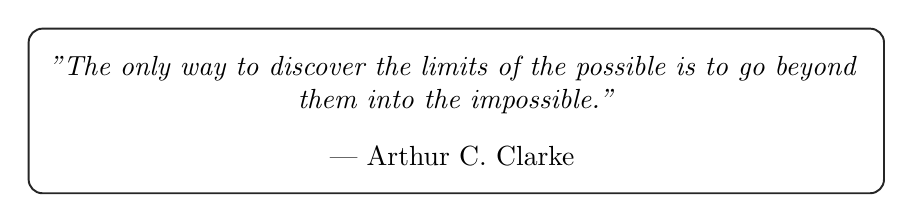
\begin{tikzpicture} % Final quote box adapted
\node[draw=rvaccent, line width=0.7pt, inner sep=10pt, rounded corners=5pt] { % Use accent color
\begin{minipage}{4in}
\centering
\textit{"The only way to discover the limits of the possible is to go beyond them into the impossible."\\} % Relevant quote
\vspace{0.3cm}
— Arthur C. Clarke
\end{minipage}
};
\end{tikzpicture}
\end{center}



\chapter*{TARGET BANK}
\thispagestyle{fancy}
\begin{center}
\Large\itshape Reference Information for Session Targets
\vspace{0.2cm}
\elegantdivider
\end{center}

\begin{mdframed}[backgroundcolor=rvlight, linewidth=0.7pt, linecolor=rvprimary, shadow=true, shadowsize=1pt, shadowcolor=graydark!40, roundcorner=3pt, innertopmargin=10pt, innerbottommargin=10pt]
\textbf{How to Use the Target Bank:} This section contains all the targets for your 90-day remote viewing practice. Each target has its own page to prevent accidental viewing of future targets. During sessions, you will be given only a reference number (e.g., "P1-02"). Only AFTER completing your session should you look up the target in this bank to verify your perceptions.

\textbf{Important:} For maximum benefit, resist the temptation to look ahead at future targets. You may wish to have a practice partner who can select random targets for you by reference number without revealing the target identity.
\end{mdframed}

\vspace{0.5cm}
\begin{center}
\begin{mdframed}[backgroundcolor=white, linewidth=0.7pt, linecolor=rvprimary, shadow=true, shadowsize=1pt, shadowcolor=graydark!40, roundcorner=3pt]
\begin{center}
\large\textbf{TARGET INDEX}
\end{center}

\textbf{Phase 1: Foundation Targets (Days 1-30)}\\
P1-01A through P1-27 \hfill pages \pageref{target:P1-01A}--\pageref{target:P1-27}

\textbf{Phase 2: Development Targets (Days 31-60)}\\
P2-31 through P2-58 \hfill pages \pageref{target:P2-31}--\pageref{target:P2-58}

\textbf{Phase 3: Advanced Targets (Days 61-90)}\\
P3-61 through P3-88 \hfill pages \pageref{target:P3-61}--\pageref{target:P3-88}
\end{mdframed}
\end{center}

% Now start the individual target pages
\cleardoublepageWithSymbol


% Phase 1 targets, one per page
\section*{Phase 1: Foundation Targets (Days 1-30)}

% Target P1-01A
\label{target:P1-01A}
\begin{center}
\Large\textbf{TARGET P1-01A}
\end{center}
\begin{mdframed}[backgroundcolor=white, linewidth=0.7pt, linecolor=rvprimary, shadow=true, shadowsize=1pt, shadowcolor=graydark!40, roundcorner=3pt]
\begin{tabular}{|p{3.5cm}|p{9cm}|}
\hline
\rowcolor{rvprimary!15}
\textbf{Target} & \textbf{Notes for Verification} \\
\hline
Conceptual: Water & Flowing, fluid, wet, may appear as waves, rivers, or other water forms \\
\hline
\end{tabular}
\end{mdframed}


% Target P1-01B
\cleardoublepageWithSymbol
\label{target:P1-01B}
\begin{center}
\Large\textbf{TARGET P1-01B}
\end{center}
\begin{mdframed}[backgroundcolor=white, linewidth=0.7pt, linecolor=rvprimary, shadow=true, shadowsize=1pt, shadowcolor=graydark!40, roundcorner=3pt]
\begin{tabular}{|p{3.5cm}|p{9cm}|}
\hline
\rowcolor{rvprimary!15}
\textbf{Target} & \textbf{Notes for Verification} \\
\hline
Conceptual: Structure & Angular, solid, man-made, building-like qualities, rigid \\
\hline
\end{tabular}
\end{mdframed}


% Target P1-01C
\cleardoublepageWithSymbol
\label{target:P1-01C}
\begin{center}
\Large\textbf{TARGET P1-01C}
\end{center}
\begin{mdframed}[backgroundcolor=white, linewidth=0.7pt, linecolor=rvprimary, shadow=true, shadowsize=1pt, shadowcolor=graydark!40, roundcorner=3pt]
\begin{tabular}{|p{3.5cm}|p{9cm}|}
\hline
\rowcolor{rvprimary!15}
\textbf{Target} & \textbf{Notes for Verification} \\
\hline
Conceptual: Land & Solid, horizontal, earthy, open space, terrain \\
\hline
\end{tabular}
\end{mdframed}


% Target P1-01D
\cleardoublepageWithSymbol
\label{target:P1-01D}
\begin{center}
\Large\textbf{TARGET P1-01D}
\end{center}
\begin{mdframed}[backgroundcolor=white, linewidth=0.7pt, linecolor=rvprimary, shadow=true, shadowsize=1pt, shadowcolor=graydark!40, roundcorner=3pt]
\begin{tabular}{|p{3.5cm}|p{9cm}|}
\hline
\rowcolor{rvprimary!15}
\textbf{Target} & \textbf{Notes for Verification} \\
\hline
Conceptual: Energy & Dynamic, moving, radiating, might appear as light or vibration \\
\hline
\end{tabular}
\end{mdframed}


% Target P1-01E
\cleardoublepageWithSymbol
\label{target:P1-01E}
\begin{center}
\Large\textbf{TARGET P1-01E}
\end{center}
\begin{mdframed}[backgroundcolor=white, linewidth=0.7pt, linecolor=rvprimary, shadow=true, shadowsize=1pt, shadowcolor=graydark!40, roundcorner=3pt]
\begin{tabular}{|p{3.5cm}|p{9cm}|}
\hline
\rowcolor{rvprimary!15}
\textbf{Target} & \textbf{Notes for Verification} \\
\hline
Conceptual: Movement & Directional flow, action, change of position, dynamic \\
\hline
\end{tabular}
\end{mdframed}


% Target P1-02
\cleardoublepageWithSymbol
\label{target:P1-02}
\begin{center}
\Large\textbf{TARGET P1-02}
\end{center}
\begin{mdframed}[backgroundcolor=white, linewidth=0.7pt, linecolor=rvprimary, shadow=true, shadowsize=1pt, shadowcolor=graydark!40, roundcorner=3pt]
\begin{tabular}{|p{3.5cm}|p{9cm}|}
\hline
\rowcolor{rvprimary!15}
\textbf{Target} & \textbf{Notes for Verification} \\
\hline
Spoon & Metal eating utensil with oval bowl and handle, curved form \\
\hline
\end{tabular}
\end{mdframed}


% Target P1-03
\cleardoublepageWithSymbol
\label{target:P1-03}
\begin{center}
\Large\textbf{TARGET P1-03}
\end{center}
\begin{mdframed}[backgroundcolor=white, linewidth=0.7pt, linecolor=rvprimary, shadow=true, shadowsize=1pt, shadowcolor=graydark!40, roundcorner=3pt]
\begin{tabular}{|p{3.5cm}|p{9cm}|}
\hline
\rowcolor{rvprimary!15}
\textbf{Target} & \textbf{Notes for Verification} \\
\hline
Ball & Spherical object, round in all dimensions, may be various sizes \\
\hline
\end{tabular}
\end{mdframed}


% Target P1-04
\cleardoublepageWithSymbol
\label{target:P1-04}
\begin{center}
\Large\textbf{TARGET P1-04}
\end{center}
\begin{mdframed}[backgroundcolor=white, linewidth=0.7pt, linecolor=rvprimary, shadow=true, shadowsize=1pt, shadowcolor=graydark!40, roundcorner=3pt]
\begin{tabular}{|p{3.5cm}|p{9cm}|}
\hline
\rowcolor{rvprimary!15}
\textbf{Target} & \textbf{Notes for Verification} \\
\hline
Orange & Spherical fruit with textured peel, orange color, citrus smell \\
\hline
\end{tabular}
\end{mdframed}


\cleardoublepageWithSymbol
% Target P1-05
\label{target:P1-05}
\begin{center}
\Large\textbf{TARGET P1-05}
\end{center}
\begin{mdframed}[backgroundcolor=white, linewidth=0.7pt, linecolor=rvprimary, shadow=true, shadowsize=1pt, shadowcolor=graydark!40, roundcorner=3pt]
\begin{tabular}{|p{3.5cm}|p{9cm}|}
\hline
\rowcolor{rvprimary!15}
\textbf{Target} & \textbf{Notes for Verification} \\
\hline
Ice Cube & Cold, clear/white, solid form of water, melts at room temperature \\
\hline
\end{tabular}
\end{mdframed}


\cleardoublepageWithSymbol
% Target P1-07
\label{target:P1-07}

\begin{center}
\Large\textbf{TARGET P1-07}
\end{center}
\begin{mdframed}[backgroundcolor=white, linewidth=0.7pt, linecolor=rvprimary, shadow=true, shadowsize=1pt, shadowcolor=graydark!40, roundcorner=3pt]
\begin{tabular}{|p{3.5cm}|p{9cm}|}
\hline
\rowcolor{rvprimary!15}
\textbf{Target} & \textbf{Notes for Verification} \\
\hline
Wooden Block & Solid cube or rectangular prism made of wood, hard texture \\
\hline
\end{tabular}
\end{mdframed}


\cleardoublepageWithSymbol
% Target P1-08
\label{target:P1-08}
\begin{center}
\Large\textbf{TARGET P1-08}
\end{center}
\begin{mdframed}[backgroundcolor=white, linewidth=0.7pt, linecolor=rvprimary, shadow=true, shadowsize=1pt, shadowcolor=graydark!40, roundcorner=3pt]
\begin{tabular}{|p{3.5cm}|p{9cm}|}
\hline
\rowcolor{rvprimary!15}
\textbf{Target} & \textbf{Notes for Verification} \\
\hline
Sandpaper & Abrasive sheet with rough texture, used for smoothing surfaces \\
\hline
\end{tabular}
\end{mdframed}


\cleardoublepageWithSymbol
% Target P1-09
\label{target:P1-09}
\begin{center}
\Large\textbf{TARGET P1-09}
\end{center}
\begin{mdframed}[backgroundcolor=white, linewidth=0.7pt, linecolor=rvprimary, shadow=true, shadowsize=1pt, shadowcolor=graydark!40, roundcorner=3pt]
\begin{tabular}{|p{3.5cm}|p{9cm}|}
\hline
\rowcolor{rvprimary!15}
\textbf{Target} & \textbf{Notes for Verification} \\
\hline
Bell & Metal object that makes ringing sound, typically dome or cup shaped \\
\hline
\end{tabular}
\end{mdframed}


\cleardoublepageWithSymbol
% Target P1-10
\label{target:P1-10}
\begin{center}
\Large\textbf{TARGET P1-10}
\end{center}
\begin{mdframed}[backgroundcolor=white, linewidth=0.7pt, linecolor=rvprimary, shadow=true, shadowsize=1pt, shadowcolor=graydark!40, roundcorner=3pt]
\begin{tabular}{|p{3.5cm}|p{9cm}|}
\hline
\rowcolor{rvprimary!15}
\textbf{Target} & \textbf{Notes for Verification} \\
\hline
Apple & Round fruit with smooth skin, typically red, green, or yellow \\
\hline
\end{tabular}
\end{mdframed}


\cleardoublepageWithSymbol
% Target P1-11
\label{target:P1-11}
\begin{center}
\Large\textbf{TARGET P1-11}
\end{center}
\begin{mdframed}[backgroundcolor=white, linewidth=0.7pt, linecolor=rvprimary, shadow=true, shadowsize=1pt, shadowcolor=graydark!40, roundcorner=3pt]
\begin{tabular}{|p{3.5cm}|p{9cm}|}
\hline
\rowcolor{rvprimary!15}
\textbf{Target} & \textbf{Notes for Verification} \\
\hline
Tall Box & Rectangular container with height greater than width, vertical emphasis \\
\hline
\end{tabular}
\end{mdframed}


\cleardoublepageWithSymbol
% Target P1-12
\label{target:P1-12}
\begin{center}
\Large\textbf{TARGET P1-12}
\end{center}
\begin{mdframed}[backgroundcolor=white, linewidth=0.7pt, linecolor=rvprimary, shadow=true, shadowsize=1pt, shadowcolor=graydark!40, roundcorner=3pt]
\begin{tabular}{|p{3.5cm}|p{9cm}|}
\hline
\rowcolor{rvprimary!15}
\textbf{Target} & \textbf{Notes for Verification} \\
\hline
Flat Plate & Thin, circular or rectangular dish with wide, flat surface \\
\hline
\end{tabular}
\end{mdframed}


\cleardoublepageWithSymbol
% Target P1-13
\label{target:P1-13}
\begin{center}
\Large\textbf{TARGET P1-13}
\end{center}
\begin{mdframed}[backgroundcolor=white, linewidth=0.7pt, linecolor=rvprimary, shadow=true, shadowsize=1pt, shadowcolor=graydark!40, roundcorner=3pt]
\begin{tabular}{|p{3.5cm}|p{9cm}|}
\hline
\rowcolor{rvprimary!15}
\textbf{Target} & \textbf{Notes for Verification} \\
\hline
Cup & Container for liquids, typically with handle, open at top \\
\hline
\end{tabular}
\end{mdframed}


\cleardoublepageWithSymbol
% Target P1-15
\label{target:P1-15}
\begin{center}
\Large\textbf{TARGET P1-15}
\end{center}
\begin{mdframed}[backgroundcolor=white, linewidth=0.7pt, linecolor=rvprimary, shadow=true, shadowsize=1pt, shadowcolor=graydark!40, roundcorner=3pt]
\begin{tabular}{|p{3.5cm}|p{9cm}|}
\hline
\rowcolor{rvprimary!15}
\textbf{Target} & \textbf{Notes for Verification} \\
\hline
Fabric Swatch & Piece of cloth/textile material, soft, flexible, may have pattern \\
\hline
\end{tabular}
\end{mdframed}


\cleardoublepageWithSymbol
% Target P1-16
\label{target:P1-16}
\begin{center}
\Large\textbf{TARGET P1-16}
\end{center}
\begin{mdframed}[backgroundcolor=white, linewidth=0.7pt, linecolor=rvprimary, shadow=true, shadowsize=1pt, shadowcolor=graydark!40, roundcorner=3pt]
\begin{tabular}{|p{3.5cm}|p{9cm}|}
\hline
\rowcolor{rvprimary!15}
\textbf{Target} & \textbf{Notes for Verification} \\
\hline
Metal Bolt & Threaded fastener with hexagonal head, made of metal \\
\hline
\end{tabular}
\end{mdframed}


\cleardoublepageWithSymbol
% Target P1-17
\label{target:P1-17}
\begin{center}
\Large\textbf{TARGET P1-17}
\end{center}
\begin{mdframed}[backgroundcolor=white, linewidth=0.7pt, linecolor=rvprimary, shadow=true, shadowsize=1pt, shadowcolor=graydark!40, roundcorner=3pt]
\begin{tabular}{|p{3.5cm}|p{9cm}|}
\hline
\rowcolor{rvprimary!15}
\textbf{Target} & \textbf{Notes for Verification} \\
\hline
Banana & Curved yellow fruit with soft interior and peel exterior \\
\hline
\end{tabular}
\end{mdframed}


\cleardoublepageWithSymbol
% Target P1-18
\label{target:P1-18}
\begin{center}
\Large\textbf{TARGET P1-18}
\end{center}
\begin{mdframed}[backgroundcolor=white, linewidth=0.7pt, linecolor=rvprimary, shadow=true, shadowsize=1pt, shadowcolor=graydark!40, roundcorner=3pt]
\begin{tabular}{|p{3.5cm}|p{9cm}|}
\hline
\rowcolor{rvprimary!15}
\textbf{Target} & \textbf{Notes for Verification} \\
\hline
Book & Bound pages with text/images, rectangular, flat \\
\hline
\end{tabular}
\end{mdframed}


\cleardoublepageWithSymbol
% Target P1-19
\label{target:P1-19}
\begin{center}
\Large\textbf{TARGET P1-19}
\end{center}
\begin{mdframed}[backgroundcolor=white, linewidth=0.7pt, linecolor=rvprimary, shadow=true, shadowsize=1pt, shadowcolor=graydark!40, roundcorner=3pt]
\begin{tabular}{|p{3.5cm}|p{9cm}|}
\hline
\rowcolor{rvprimary!15}
\textbf{Target} & \textbf{Notes for Verification} \\
\hline
Coffee Grounds & Dark granular substance with strong aroma, used for brewing \\
\hline
\end{tabular}
\end{mdframed}


\cleardoublepageWithSymbol
% Target P1-20
\label{target:P1-20}
\begin{center}
\Large\textbf{TARGET P1-20}
\end{center}
\begin{mdframed}[backgroundcolor=white, linewidth=0.7pt, linecolor=rvprimary, shadow=true, shadowsize=1pt, shadowcolor=graydark!40, roundcorner=3pt]
\begin{tabular}{|p{3.5cm}|p{9cm}|}
\hline
\rowcolor{rvprimary!15}
\textbf{Target} & \textbf{Notes for Verification} \\
\hline
Small Plant & Living botanical organism in pot, green, growing upward \\
\hline
\end{tabular}
\end{mdframed}


\cleardoublepageWithSymbol
% Target P1-21
\label{target:P1-21}
\begin{center}
\Large\textbf{TARGET P1-21}
\end{center}
\begin{mdframed}[backgroundcolor=white, linewidth=0.7pt, linecolor=rvprimary, shadow=true, shadowsize=1pt, shadowcolor=graydark!40, roundcorner=3pt]
\begin{tabular}{|p{3.5cm}|p{9cm}|}
\hline
\rowcolor{rvprimary!15}
\textbf{Target} & \textbf{Notes for Verification} \\
\hline
Geometric Shape & Simple form like triangle, square, circle, or star \\
\hline
\end{tabular}
\end{mdframed}


\cleardoublepageWithSymbol
% Target P1-22
\label{target:P1-22}
\begin{center}
\Large\textbf{TARGET P1-22}
\end{center}
\begin{mdframed}[backgroundcolor=white, linewidth=0.7pt, linecolor=rvprimary, shadow=true, shadowsize=1pt, shadowcolor=graydark!40, roundcorner=3pt]
\begin{tabular}{|p{3.5cm}|p{9cm}|}
\hline
\rowcolor{rvprimary!15}
\textbf{Target} & \textbf{Notes for Verification} \\
\hline
Smooth Stone & Natural rock with rounded edges, cool to touch \\
\hline
\end{tabular}
\end{mdframed}


\cleardoublepageWithSymbol
% Target P1-23
\label{target:P1-23}
\begin{center}
\Large\textbf{TARGET P1-23}
\end{center}
\begin{mdframed}[backgroundcolor=white, linewidth=0.7pt, linecolor=rvprimary, shadow=true, shadowsize=1pt, shadowcolor=graydark!40, roundcorner=3pt]
\begin{tabular}{|p{3.5cm}|p{9cm}|}
\hline
\rowcolor{rvprimary!15}
\textbf{Target} & \textbf{Notes for Verification} \\
\hline
Glass of Water & Transparent container holding clear liquid \\
\hline
\end{tabular}
\end{mdframed}


\cleardoublepageWithSymbol
% Target P1-24
\label{target:P1-24}
\begin{center}
\Large\textbf{TARGET P1-24}
\end{center}
\begin{mdframed}[backgroundcolor=white, linewidth=0.7pt, linecolor=rvprimary, shadow=true, shadowsize=1pt, shadowcolor=graydark!40, roundcorner=3pt]
\begin{tabular}{|p{3.5cm}|p{9cm}|}
\hline
\rowcolor{rvprimary!15}
\textbf{Target} & \textbf{Notes for Verification} \\
\hline
Photo of Car & Image of automobile, complex man-made vehicle \\
\hline
\end{tabular}
\end{mdframed}


\cleardoublepageWithSymbol
% Target P1-25A
\label{target:P1-25A}
\begin{center}
\Large\textbf{TARGET P1-25A}
\end{center}
\begin{mdframed}[backgroundcolor=white, linewidth=0.7pt, linecolor=rvprimary, shadow=true, shadowsize=1pt, shadowcolor=graydark!40, roundcorner=3pt]
\begin{tabular}{|p{3.5cm}|p{9cm}|}
\hline
\rowcolor{rvprimary!15}
\textbf{Target} & \textbf{Notes for Verification} \\
\hline
Inside Box & Enclosed, contained perspective from within a box structure \\
\hline
\end{tabular}
\end{mdframed}


\cleardoublepageWithSymbol
% Target P1-25B
\label{target:P1-25B}
\begin{center}
\Large\textbf{TARGET P1-25B}
\end{center}
\begin{mdframed}[backgroundcolor=white, linewidth=0.7pt, linecolor=rvprimary, shadow=true, shadowsize=1pt, shadowcolor=graydark!40, roundcorner=3pt]
\begin{tabular}{|p{3.5cm}|p{9cm}|}
\hline
\rowcolor{rvprimary!15}
\textbf{Target} & \textbf{Notes for Verification} \\
\hline
Outside Box & External view of a container, seeing from outside \\
\hline
\end{tabular}
\end{mdframed}


\cleardoublepageWithSymbol
% Target P1-26
\label{target:P1-26}
\begin{center}
\Large\textbf{TARGET P1-26}
\end{center}
\begin{mdframed}[backgroundcolor=white, linewidth=0.7pt, linecolor=rvprimary, shadow=true, shadowsize=1pt, shadowcolor=graydark!40, roundcorner=3pt]
\begin{tabular}{|p{3.5cm}|p{9cm}|}
\hline
\rowcolor{rvprimary!15}
\textbf{Target} & \textbf{Notes for Verification} \\
\hline
Warm Mug & Heat-emitting drinking vessel, radiating warmth \\
\hline
\end{tabular}
\end{mdframed}


\cleardoublepageWithSymbol
% Target P1-27
\label{target:P1-27}
\begin{center}
\Large\textbf{TARGET P1-27}
\end{center}
\begin{mdframed}[backgroundcolor=white, linewidth=0.7pt, linecolor=rvprimary, shadow=true, shadowsize=1pt, shadowcolor=graydark!40, roundcorner=3pt]
\begin{tabular}{|p{3.5cm}|p{9cm}|}
\hline
\rowcolor{rvprimary!15}
\textbf{Target} & \textbf{Notes for Verification} \\
\hline
Toy Figure & Small human or character representation, possibly plastic \\
\hline
\end{tabular}
\end{mdframed}

\cleardoublepageWithSymbol

% Phase 2 targets, one per page
\section*{Phase 2: Development Targets (Days 31-60)}

% Target P2-31
\label{target:P2-31}
\begin{center}
\Large\textbf{TARGET P2-31}
\end{center}
\begin{mdframed}[backgroundcolor=white, linewidth=0.7pt, linecolor=rvprimary, shadow=true, shadowsize=1pt, shadowcolor=graydark!40, roundcorner=3pt]
\begin{tabular}{|p{3.5cm}|p{9cm}|}
\hline
\rowcolor{rvprimary!15}
\textbf{Target} & \textbf{Notes for Verification} \\
\hline
Outdoor Scene & Natural setting with field and single tree, open space \\
\hline
\end{tabular}
\end{mdframed}


\cleardoublepageWithSymbol
% Target P2-32
\label{target:P2-32}
\begin{center}
\Large\textbf{TARGET P2-32}
\end{center}
\begin{mdframed}[backgroundcolor=white, linewidth=0.7pt, linecolor=rvprimary, shadow=true, shadowsize=1pt, shadowcolor=graydark!40, roundcorner=3pt]
\begin{tabular}{|p{3.5cm}|p{9cm}|}
\hline
\rowcolor{rvprimary!15}
\textbf{Target} & \textbf{Notes for Verification} \\
\hline
Hospital & Medical facility with multiple rooms, staff in uniforms, medical equipment \\
\hline
\end{tabular}
\end{mdframed}


\cleardoublepageWithSymbol
% Target P2-33
\label{target:P2-33}
\begin{center}
\Large\textbf{TARGET P2-33}
\end{center}
\begin{mdframed}[backgroundcolor=white, linewidth=0.7pt, linecolor=rvprimary, shadow=true, shadowsize=1pt, shadowcolor=graydark!40, roundcorner=3pt]
\begin{tabular}{|p{3.5cm}|p{9cm}|}
\hline
\rowcolor{rvprimary!15}
\textbf{Target} & \textbf{Notes for Verification} \\
\hline
School & Educational facility with classrooms, desks, chalkboards/whiteboards \\
\hline
\end{tabular}
\end{mdframed}

\cleardoublepageWithSymbol
% Target P2-34 (Your selection example)
\label{target:P2-34}
\begin{center}
\Large\textbf{TARGET P2-34}
\end{center}
\begin{mdframed}[backgroundcolor=white, linewidth=0.7pt, linecolor=rvprimary, shadow=true, shadowsize=1pt, shadowcolor=graydark!40, roundcorner=3pt]
\begin{tabular}{|p{3.5cm}|p{9cm}|}
\hline
\rowcolor{rvprimary!15}
\textbf{Target} & \textbf{Notes for Verification} \\
\hline
Simple Object & Something Else you select - A basic object with clear form \\
\hline
\end{tabular}

\vspace{0.3cm}
\textbf{Selection Notes:} Choose any simple physical object with clear boundaries and form. Examples might include a pen, small toy, tool, or household item. For best results, select something with distinctive characteristics but avoid objects with strong personal associations.

\vspace{0.2cm}
Selected object: \rule{4in}{0.4pt}

\vspace{0.2cm}
Key identifying features: \rule{4in}{0.4pt}
\end{mdframed}


\cleardoublepageWithSymbol
% Target P2-35
\label{target:P2-35}
\begin{center}
\Large\textbf{TARGET P2-35}
\end{center}
\begin{mdframed}[backgroundcolor=white, linewidth=0.7pt, linecolor=rvprimary, shadow=true, shadowsize=1pt, shadowcolor=graydark!40, roundcorner=3pt]
\begin{tabular}{|p{3.5cm}|p{9cm}|}
\hline
\rowcolor{rvprimary!15}
\textbf{Target} & \textbf{Notes for Verification} \\
\hline
Library & Room or building filled with books on shelves, reading areas \\
\hline
\end{tabular}
\end{mdframed}


\cleardoublepageWithSymbol
% Target P2-36
\label{target:P2-36}
\begin{center}
\Large\textbf{TARGET P2-36}
\end{center}
\begin{mdframed}[backgroundcolor=white, linewidth=0.7pt, linecolor=rvprimary, shadow=true, shadowsize=1pt, shadowcolor=graydark!40, roundcorner=3pt]
\begin{tabular}{|p{3.5cm}|p{9cm}|}
\hline
\rowcolor{rvprimary!15}
\textbf{Target} & \textbf{Notes for Verification} \\
\hline
River & Natural flowing water body, winding through landscape \\
\hline
\end{tabular}
\end{mdframed}


% Continue with remaining Phase 2 targets...
\cleardoublepageWithSymbol

% Phase 3 targets examples (select few)
\section*{Phase 3: Advanced Targets (Days 61-90)}

% Target P3-61
\label{target:P3-61}
\begin{center}
\Large\textbf{TARGET P3-61}
\end{center}
\begin{mdframed}[backgroundcolor=white, linewidth=0.7pt, linecolor=rvprimary, shadow=true, shadowsize=1pt, shadowcolor=graydark!40, roundcorner=3pt]
\begin{tabular}{|p{3.5cm}|p{9cm}|}
\hline
\rowcolor{rvprimary!15}
\textbf{Target} & \textbf{Notes for Verification} \\
\hline
Car Engine & Complex mechanical system with multiple parts, the power center of a vehicle \\
\hline
\end{tabular}
\end{mdframed}


\cleardoublepageWithSymbol
% Target P3-62
\label{target:P3-62}
\begin{center}
\Large\textbf{TARGET P3-62}
\end{center}
\begin{mdframed}[backgroundcolor=white, linewidth=0.7pt, linecolor=rvprimary, shadow=true, shadowsize=1pt, shadowcolor=graydark!40, roundcorner=3pt]
\begin{tabular}{|p{3.5cm}|p{9cm}|}
\hline
\rowcolor{rvprimary!15}
\textbf{Target} & \textbf{Notes for Verification} \\
\hline
Park Water Feature & Fountain, pond, or waterfall in public recreational space \\
\hline
\end{tabular}
\end{mdframed}


\cleardoublepageWithSymbol
% Target P3-63
\label{target:P3-63}
\begin{center}
\Large\textbf{TARGET P3-63}
\end{center}
\begin{mdframed}[backgroundcolor=white, linewidth=0.7pt, linecolor=rvprimary, shadow=true, shadowsize=1pt, shadowcolor=graydark!40, roundcorner=3pt]
\begin{tabular}{|p{3.5cm}|p{9cm}|}
\hline
\rowcolor{rvprimary!15}
\textbf{Target} & \textbf{Notes for Verification} \\
\hline
Building Structure & Architectural construction with rooms, foundation, roof \\
\hline
\end{tabular}
\end{mdframed}


\cleardoublepageWithSymbol
% Target P3-64
\label{target:P3-64}
\begin{center}
\Large\textbf{TARGET P3-64}
\end{center}
\begin{mdframed}[backgroundcolor=white, linewidth=0.7pt, linecolor=rvprimary, shadow=true, shadowsize=1pt, shadowcolor=graydark!40, roundcorner=3pt]
\begin{tabular}{|p{3.5cm}|p{9cm}|}
\hline
\rowcolor{rvprimary!15}
\textbf{Target} & \textbf{Notes for Verification} \\
\hline
Person Running & Human in athletic motion, legs in stride, arms pumping \\
\hline
\end{tabular}
\end{mdframed}

\cleardoublepageWithSymbol

% Target P3-65 (Your selection example)
\label{target:P3-65}
\begin{center}
\Large\textbf{TARGET P3-65}
\end{center}
\begin{mdframed}[backgroundcolor=white, linewidth=0.7pt, linecolor=rvprimary, shadow=true, shadowsize=1pt, shadowcolor=graydark!40, roundcorner=3pt]
\begin{tabular}{|p{3.5cm}|p{9cm}|}
\hline
\rowcolor{rvprimary!15}
\textbf{Target} & \textbf{Notes for Verification} \\
\hline
Interesting Location & A place YOU select - A noteworthy place with distinctive features \\
\hline
\end{tabular}

\vspace{0.3cm}
\textbf{Selection Notes:} Select a location with distinctive characteristics and features. This could be a landmark, natural wonder, architectural site, or other place of interest. Choose something with unique energy or qualities that would make it an engaging remote viewing target.

\vspace{0.2cm}
Selected location: \\ \rule{0pt}{1in}

\vspace{0.2cm}
Key identifying features: \\ \rule{0pt}{1in}

\vspace{0.2cm}
What makes this location distinctive:\\
\rule{0pt}{1in}
\end{mdframed}

\cleardoublepageWithSymbol

% Target P3-85 (Practice partner selection)
\label{target:P3-85}
\begin{center}
\Large\textbf{TARGET P3-85}
\end{center}
\begin{mdframed}[backgroundcolor=white, linewidth=0.7pt, linecolor=rvprimary, shadow=true, shadowsize=1pt, shadowcolor=graydark!40, roundcorner=3pt]
\begin{tabular}{|p{3.5cm}|p{9cm}|}
\hline
\rowcolor{rvprimary!15}
\textbf{Target} & \textbf{Notes for Verification} \\
\hline
Assistant's Selection & Target selected by your practice partner \\
\hline
\end{tabular}

\vspace{0.3cm}
\textbf{Selection Notes:} This target should be chosen by your practice partner without revealing any information to you. After your session is complete, they will provide the feedback for verification.

\vspace{0.2cm}
\textbf{For Practice Partner:}\\
Selected target (describe in detail): \rule{0pt}{1in}


\vspace{0.2cm}
Key identifying features:\\
\rule{0pt}{1in}
\end{mdframed}
\cleardoublepageWithSymbol

% Final instructions sections

\section*{Practice Partner Instructions}
\begin{mdframed}[backgroundcolor=rvlight, linewidth=0.7pt, linecolor=rvprimary, shadow=true, shadowsize=1pt, shadowcolor=graydark!40, roundcorner=3pt]
If working with a practice partner, they can help create truly blind remote viewing conditions:

\begin{enumerate}
\item Partner selects a target reference from the Target Bank without revealing which one
\item Partner writes only the reference number (e.g., "P2-45") on an envelope or paper
\item You conduct your remote viewing session using only the reference number
\item Afterward, your partner reveals the target for feedback and analysis
\end{enumerate}

For advanced practice (Days 85+), partners can select their own targets not in this bank, assign them a unique reference number, and reveal them only after your session.
\end{mdframed}

\section*{Creating Additional Targets}
\begin{mdframed}[backgroundcolor=rvlight, linewidth=0.7pt, linecolor=rvprimary, shadow=true, shadowsize=1pt, shadowcolor=graydark!40, roundcorner=3pt]
To extend your practice beyond the 90-day protocol:

\begin{enumerate}
\item Collect interesting photos, objects, or locations
\item Assign each a unique reference number (e.g., "X-001", "X-002")
\item Have a practice partner manage these targets to ensure blind viewing
\item Consider categories like: landmarks, natural features, historical events, art objects, machinery, or everyday items
\end{enumerate}

Remember that the best targets for remote viewing practice have distinctive characteristics, clear boundaries, and some level of uniqueness or interest.
\end{mdframed}

\begin{quotebox}
"The target exists independently of your awareness of it. Trust the protocol to guide your perception to its reality." — Remote Viewing Principle
\end{quotebox}

\end{document}
